%%%%%%%%%%%%%%%%%%%%%%%%%%%%%%%%%%%%%%%%%%%%%%%%%%%%%%%%%%%%
%%% ELIFE ARTICLE TEMPLATE
%%%%%%%%%%%%%%%%%%%%%%%%%%%%%%%%%%%%%%%%%%%%%%%%%%%%%%%%%%%%
%%% PREAMBLE 
\documentclass[9pt,lineno]{elife}
% Use the onehalfspacing option for 1.5 line spacing
% Use the doublespacing option for 2.0 line spacing
% Please note that these options may affect formatting.
% Additionally, the use of the \newcommand function should be limited.


\usepackage{lipsum} % Required to insert dummy text
\usepackage[version=4]{mhchem}
\usepackage{siunitx}
\usepackage[export]{adjustbox}
\usepackage{float}
\DeclareSIUnit\Molar{M}

\newcommand{\jdbcomment}[1]{\emph{\color{red} [#1]}}

\newfloat{suppfile}{thp}{lofsupfile}
%\renewcommand{\thesuppfile}{Supplementary file \arabic{suppfile}}
\floatname{suppfile}{Supplementary file}

%%%%%%%%%%%%%%%%%%%%%%%%%%%%%%%%%%%%%%%%%%%%%%%%%%%%%%%%%%%%
%%% ARTICLE SETUP
%%%%%%%%%%%%%%%%%%%%%%%%%%%%%%%%%%%%%%%%%%%%%%%%%%%%%%%%%%%%
\title{Single-cell virus sequencing of influenza variants that trigger innate immunity}

\author[1]{Alistair B. Russell}
\author[1,2,3*]{Jesse D. Bloom}
\affil[1]{Basic Sciences Division and Computational Biology Program, Fred Hutchinson Cancer Research Center, Seattle, United States}
\affil[2]{Department of Genome Sciences, University of Washington, Seattle, United States}
\affil[3]{Howard Hughes Medical Institute, Fred Hutchinson Cancer Research Center, Seattle, United States}

\corr{jbloom@fredhutch.org}{JDB}

%%%%%%%%%%%%%%%%%%%%%%%%%%%%%%%%%%%%%%%%%%%%%%%%%%%%%%%%%%%%
%%% ARTICLE START
%%%%%%%%%%%%%%%%%%%%%%%%%%%%%%%%%%%%%%%%%%%%%%%%%%%%%%%%%%%%

\begin{document}

\maketitle

\begin{abstract}
The outcome of viral infection is extremely heterogeneous at the cellular level, and many viruses trigger innate immunity in only a fraction of infected cells. 
Here we develop an approach to determine how the genetic variation inherent in viral populations contributes to this heterogeneity.
We simultaneously determine the cellular transcriptome and full sequences of all viral genes in hundreds of influenza-infected cells.
Infections that trigger immunity are associated with several features: absence of the gene encoding the virus's primary immune antagonist, internal deletions in viral polymerase genes, and point mutations in viral proteins involved in replication and nuclear export. 
However, immune activation remains stochastic in cells infected by viruses with these genetic lesions, and sometimes occurs even in cells infected with fully wildtype virions.
Overall, our work shows that viral genetic variation substantially contributes to but does not fully explain heterogeneity in infection outcome and immune activation.
\end{abstract}


\section{Introduction}

\citep{russell2018extreme} and \citep{steuerman2018dissection}.

\clearpage
\section{Results}

\subsection{A method to obtain the complete genotypes of the virions infecting single cells that do and do not express IFN}

Two challenges:

IFN expression is rare in infected cells (\FIG{IFNrare}).
Apparent in single-cell \textit{in vitro}~\citep{russell2018extreme}, single-cell \textit{in vivo}~\citep{steuerman2018dissection}, and reporter assays by others~\citep{killip2017single} and ourselves (\FIG{IFNrare}).

%%% start IFNrare figure %%%
\begin{figure}
\centerline{
{\bf \Large A}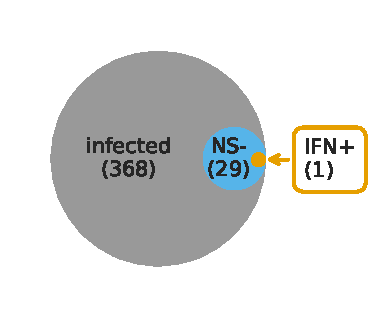
\includegraphics[width=0.25\textwidth,valign=t]{figures/IFN_stochastic/RussellVenn/venn_diagram.pdf}
\hspace{0.05\textwidth}
{\bf \Large B}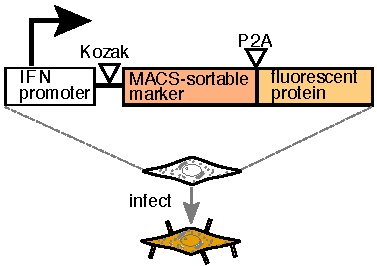
\includegraphics[width=0.35\textwidth,valign=t]{figures/IFN_stochastic/IFN_reporter/IFN_reporter.pdf}
\hspace{0.05\textwidth}
{\bf \Large C} \jdbcomment{ADD FIGURE PANEL}
}
\caption{
Triggering of IFN production is rare in influenza-infected cells.
{\bf (A)} Number of influenza-infected and IFN+ cells in our prior single-cell study of influenza infection of A549 cells.
The Venn diagram shows data aggregated over all samples from \citet{russell2018extreme}.
{\bf (B)} Creation of an A549 reporter cell line to efficiently identify single cells expressing IFN.
The cells are engineered to contain an IFN promoter that drives expression of a fluorescent protein and cell-surface protein amenable to MACS (magnetic-activated cell sorting).
We created reporter cell lines with both type I (IFN-$\beta$) and type III (IFN-$\lambda$) promoters (\FIGDATA[IFNrare]{reporter_sequences}).
The reporters were efficiently activated when infected with a virus known to potently induce IFN (\FIGSUPP[IFNrare]{reporter_validation}).
Expression of type I and type III IFN is highly correlated in the reporter cell lines upon infection with influenza virus (\FIGSUPP[IFNrare]{type_I_vs_III}).
{\bf (C)}
Frequency of IFN induction upon infection with the influenza virus stocks used in this paper as quantified using the reporter cell lines.
\jdbcomment{This should be a simple figure, such as a plot that just shows the fraction IFN+ among flu infected cells for the virus stocks we use, plus positive and negative controls.
Then put detailed flow data in \FIGSUPP[IFNrare]{flow}. }
}
\label{fig:IFNrare}

\figsupp[Validation of IFN reporter cell lines.]
{To validate the IFN reporter cell lines, they were infected at high MOI with the Cantell strain of Sendai virus, which strongly activates IFN expression~\citep{strahle2006sendai}.
Activation of the IFN reporter was then monitored by flow cytometry using the marker indicated at the bottom of each plot (either a fluorescent protein or antibody staining for the cell-surface LNGFR).
Sendai infection efficiently activated the IFN reporter in all cases, with the strongest signal for the IFN-$\lambda$ reporter driving ZsGreen.
}
{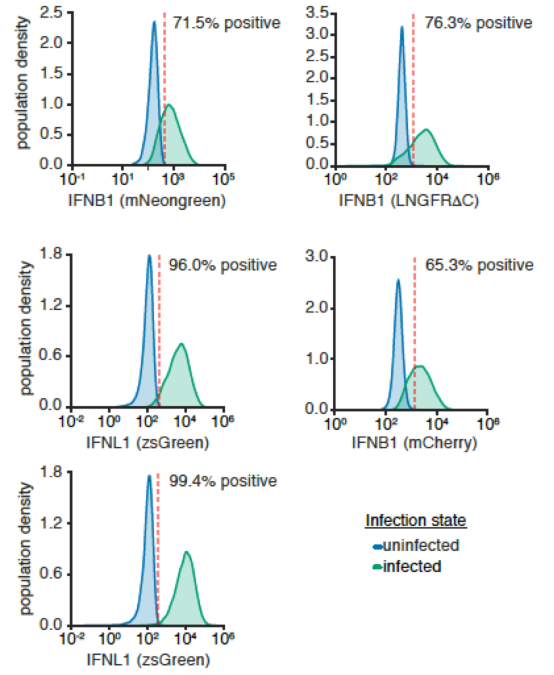
\includegraphics[width=0.5\textwidth]{figures/IFN_stochastic/IFN_reporter/Sendai_validation.pdf}}
\label{figsupp:reporter_validation}

\figsupp[Expression of type I and type III IFN are highly correlated in influenza-infected A549 cells.]
{A549 cells were dually transduced with the IFN-$\beta$ and IFN-$\lambda$ reporters driving expression of mCherry and ZsGreen, respectively.
The cells were then infected with two different stocks of ``wildtype'' WSN influenza, or stocks with a deletion in PB1 or stop codons in NS1 (described later in the paper).
After 13 hours, cells were analyzed by flow cytometry.
As shown in the FACS plots, expression of the IFN-$\beta$ and IFN-$\lambda$ reporters is highly correlated in all cases.}
{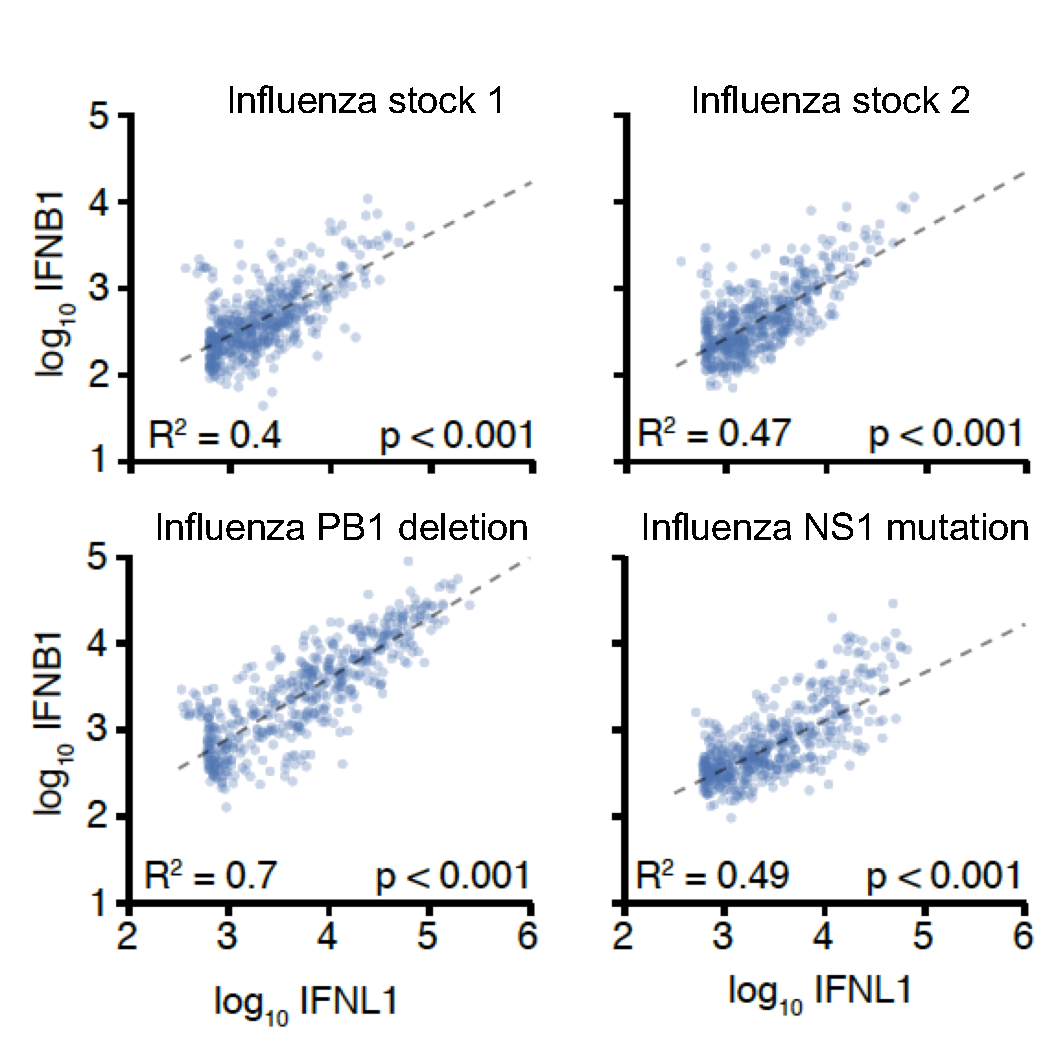
\includegraphics[width=0.5\textwidth]{figures/IFN_stochastic/IFN_reporter/IFNbeta_IFN_lambda_correlated.pdf}}
\label{figsupp:type_I_vs_III}

\figsupp[Full flow cytometry data for \FIG{IFNrare}C.]
{\jdbcomment{ADD CAPTION}}
{\jdbcomment{ADD FIGURE}}
\label{figsupp:flow}

\figsupp[Few cells express detectable IFN in the single-cell analysis influenza-infected mice by \citet{steuerman2018dissection}.]
{A re-analysis of the data from \citet{steuerman2018dissection}'s single-cell mRNA-sequencing of cells from influenza-infected mice shows that only 5 of 1220 virus-infected cells express \emph{detectable} type I or type III IFN transcripts \textit{in vivo}.
Specifically, we downloaded the data from \citet{steuerman2018dissection} and identified influenza-infected cells using calling criteria similar to those described in \citet{steuerman2018dissection}.
Here we show statistics for the cells from the influenza-infected wildtype C57BL/6J mice, which were collected at 48 hours (two replicates) or 72 hours (one replicate)---we do not show cells from the control mice.
As shown in the left-most panel, the sequencing depth of \citet{steuerman2018dissection} was quite low, with only $\sim$1,500 mRNA counts per cell on average (this is 10 to 15-fold lower than the sequencing depth in \citet{russell2018extreme} and the current study, respectively).
An important caveat is that this low sequencing depth could lead to a simple failure to detect IFN transcripts in some cells.
Nonetheless, there is detectable expression of key interferon-stimulated gene (ISG) mRNAs in the majority of infected cells (the middle panel shows the total counts of IFIT1, ISG15, CCL5, and Mx1).
However, only 5 of 1220 cells express any detectable type I (IFN-$\alpha$ and IFN-$\beta$) or type III (IFN-$\lambda$) mRNAs, and only at low levels.
The full code that performs the re-analysis shown in this figure is at \url{https://github.com/jbloomlab/IFNsorted_flu_single_cell/tree/master/paper/figures/IFN_stochastic/SteuermanReanalysis/}.
}
{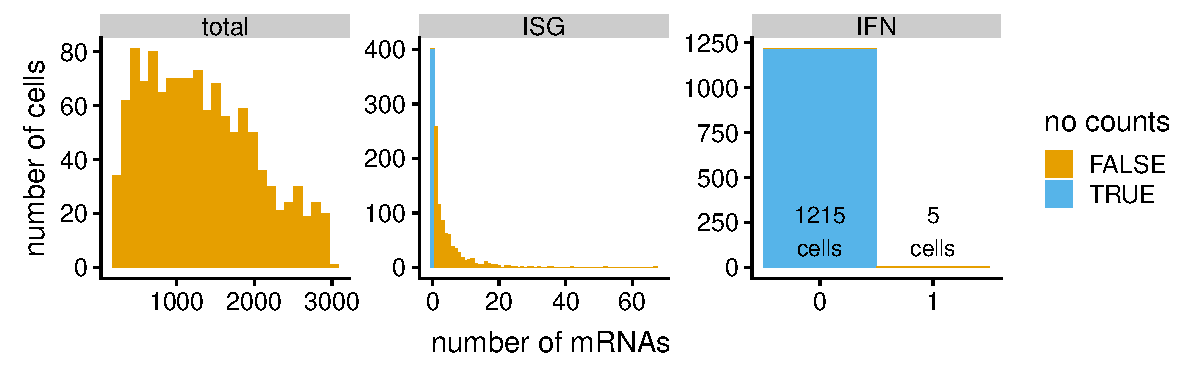
\includegraphics[width=\textwidth]{figures/IFN_stochastic/SteuermanReanalysis/plots/p_mRNA_counts.pdf}}
\label{figsupp:mice}

\figdata{Sequences of the reporters schematized in \FIG{IFNrare}B.
The MACS sortable surface marker is a truncated LNGFR.
For the IFN-$\beta$ reporter, the fluorescent protein is mNeonGreen.
For the IFN-$\lambda$ (IL29) reporter, the fluorescent protein is ZsGreen.
The sequences of plasmids carrying these reporters are at \url{https://github.com/jbloomlab/IFNsorted_flu_single_cell/tree/master/paper/figures/IFN_stochastic/IFN_reporter/1517_pHAGE2_IFNbeta_prom_LNGFR_P2A_mNeongreen.gb} and \url{https://github.com/jbloomlab/IFNsorted_flu_single_cell/tree/master/paper/figures/IFN_stochastic/IFN_reporter/1767_pHAGE2_IL29_promnkozak_LNGFR_P2A_zsGreen.gb}.
}
\label{figdata:reporter_sequences}

\end{figure}
%%% end IFNrare figure %%%

All past single-cell transcriptomics of viral infected cells~\citep{russell2018extreme,zanini2018single,steuerman2018dissection,zanini2018virus} have focused on counting the number of viral transcripts rather than determining their full sequences.
We came up with a scheme to determine full genotypes of infecting viruses in IFN+ cells (\FIG{experiment}).

%%% start approach figure
\begin{figure}
\begin{fullwidth}

\hspace{0.04in} {\bf A} 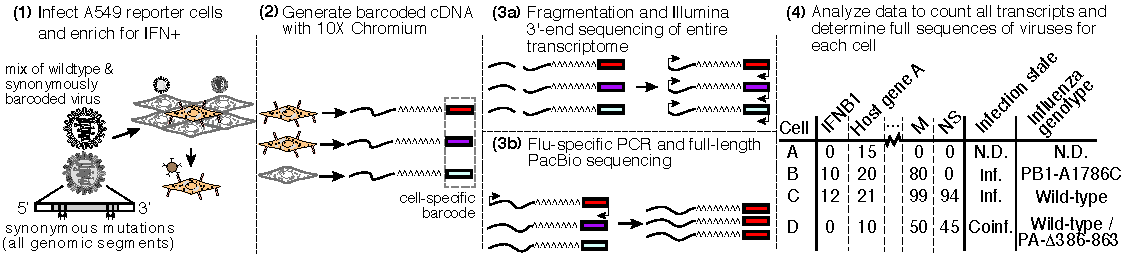
\includegraphics[width=0.9\linewidth, valign=t]{figures/WorkflowSchematic/SchematicForPaper.pdf}
\vspace{0.1in}

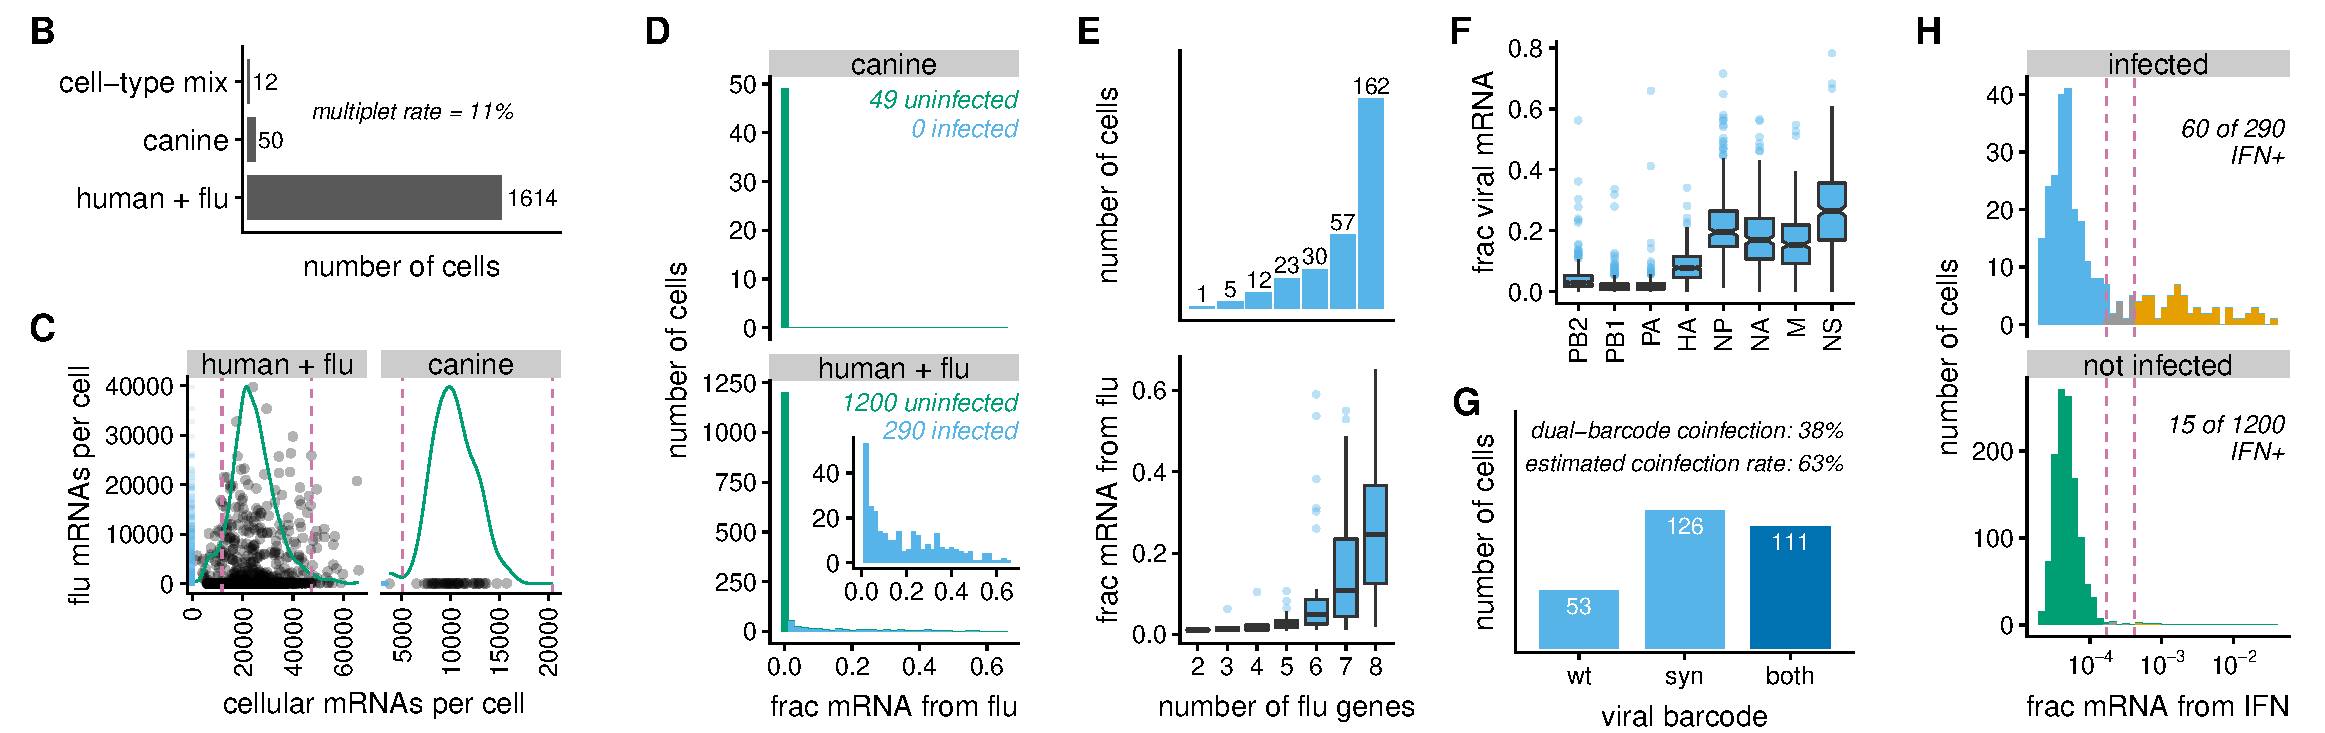
\includegraphics[width=\linewidth, clip=false]{figures/single_cell_figures/p_cell_summary.pdf}

\caption{
Single-cell virus sequencing of influenza infections that induce IFN.
{\bf (A)} Experimental workflow.
(1) IFN reporter A549 cells are infected with a mix of wildtype virus and virus carrying synonymous mutations at both ends of each gene segment.
IFN+ cells are enriched by MACS, and pooled with non-enriched cells and uninfected canine cells that serve as an internal control for multiplets and mRNA leakage.
(2) The mRNAs from individual cells are tagged with cell-specific barcodes using a 10X Chromium device.
(3) The entire cellular transcriptomes are quantified using the standard single-cell mRNA-seq protocol, and viral genes are enriched by influenza-specific PCR and fully sequenced by PacBio.
(4) The result is a matrix giving the expression of each gene in each cell, as well as the full sequences of the viral genes in infected cells.
{\bf (B)} Number of cells for which transcriptomes were obtained.
Most transcriptomes are from human cells, but a few are from the uninfected canine cells spiked into the experiment as a control.
From the transcriptomes with both human and canine transcripts, we estimate~\citep{bloom2018estimating} that $\approx$11\% of the captured cells are actually multiplets in which more than one cell was captured in an emulsion. 
These cross-celltype multiplets are excluded from subsequent analyses.
{\bf (C)} The number of cellular and viral mRNAs detected for each cell is plotted as a point.
Green lines show the distribution of cellular mRNAs per cell, and the blue rug plot at the left of each panel shows the distribution of viral mRNAs per cell.
Cells outside the dashed magenta lines have unusually low or high amounts of cellular mRNA (possibly low-quality emulsions or multiplets), and are excluded from subsequent analyses.
{\bf (D)} Distribution across cells of the fraction of all mRNA derived from influenza.
Cells called as infected are in blue, while other cells are in green.
The inset shows the amount of viral mRNA among the human cells called as infected.
{\bf (E)} The number of influenza genes detected per infected cell, and the amount of viral mRNA in cells expressing each number of viral genes.
The majority of cells express all eight gene segments, but a substantial minority fail to express at least one gene.
\FIGSUPP[experiment]{frac_has_gene} shows the frequency that each viral gene is detected in infected cells.
{\bf (F)} Relative expression of viral genes among infected cells.
{\bf (G)} The number of cells infected with wildtype virus, synonymously barcoded virus, or both.
From the cells infected with both viral barcodes, we estimate~\citep{bloom2018estimating} that 63\% of infected cells are co-infected.
{\bf (H)} Fraction of cellular mRNA derived from type I or type III IFN across all cells, faceted by whether the cells are infected.
Cells to the left of the first dashed magenta line are classified as IFN-, and cells to the right of the second line are classified as IFN+.
We grouped type I and type III IFN together because their expression is highly correlated (\FIGSUPP[experiment]{type_I_III_correlation}).
Many cells that do not express IFN itself still express interferon-stimulated genes (\FIGSUPP[experiment]{ISG}).
}
\label{fig:experiment}

\figsupp[Fraction of infected cells that detectably express each influenza gene.]
{Bars show the fraction of infected cells that are called as expressing each viral gene.
The gray dashed line is at one (the fraction that would be observed if all viral genes are expressed in all infected cells).
Each viral gene is detected in $\approx$80-90\% of the infected cells, roughly in line with prior estimates~\citep{brooke2013most, heldt2015single, dou2017analysis, russell2018extreme}.
The exception is NP, which is detected in virtually all infected cells.
The much higher frequency of detecting NP could reflect a biological phenomenon, or it could be because cells lacking NP tend to have much lower viral gene expression overall and so are not reliably called as being infected in our experiments and analysis.}
{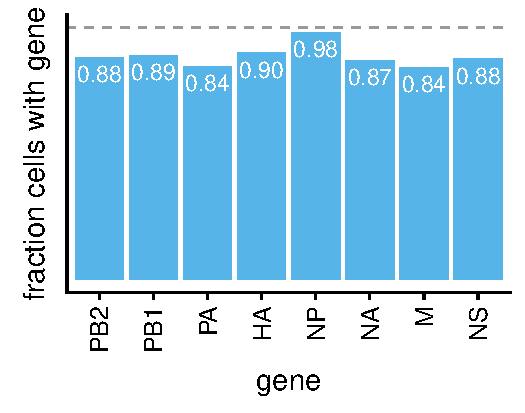
\includegraphics[width=0.5\textwidth]{figures/single_cell_figures/p_frac_has_gene.pdf}}
\label{figsupp:frac_has_gene}

\figsupp[Expression of type I and type III IFN genes is highly correlated in single cells in our experiments.]
{The correlation between the fraction of cellular mRNA derived from type I (IFN-$\alpha$ and IFN-$\beta$) and type III (IFN-$\lambda$) IFN in the A549 cells in our experiments.
Each point represents a single cell.
The plots are faceted by whether the cells are called as infected, and the Pearson correlation coefficient is shown.
Because type I and type III IFN expression are highly correlated, for the remainder of the paper we group them together and refer to their combined expression as the level of IFN.
}
{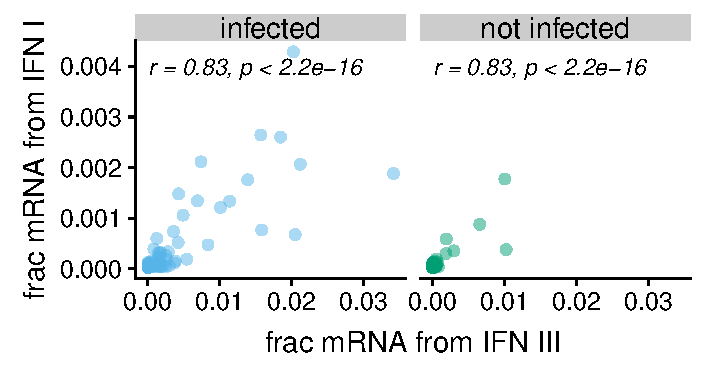
\includegraphics[width=0.7\textwidth]{figures/single_cell_figures/p_ifn_genes_corr.pdf}}
\label{figsupp:type_I_III_correlation}

\figsupp[Expression of interferon-stimulated genes (ISGs).]
{
For each cell, we quantified ISG expression as the total fraction of cellular mRNAs derived from four prototypical ISGs that are highly expressed A549 cells (IFIT1, ISG15, CCL5, and Mx1). 
{\bf (A)} The histograms show the distribution of ISG expression taken across infected (top) and uninfected (bottom) cells.
We heuristically classify as ISG+ cells with $>10^{-3}$ of their cellular mRNA from ISGs, and color these cells red.
Comparison to \FIG{experiment}H shows that substantially more cells are ISG+ than IFN+, both among infected and uninfected cells.
This is probably because paracrine signaling leads to ISG expression in some cells that are not themselves expressing IFN.
{\bf (B)} The correlation between the fraction of cellular mRNA derived from IFN and from ISGs.
Each point represents a single cell, and the Pearson correlation coefficient is shown.
IFN and ISG expression is more correlated for infected than uninfected cells, probably because in the latter the ISG expression is often due to paracrine signaling that does not induce expression of IFN itself.
But among both the infected and uninfected populations, there are many cells with high expression of ISGs and little expression of IFN, but very few cells that express high levels of IFN without also substantially expressing ISGs.
}
{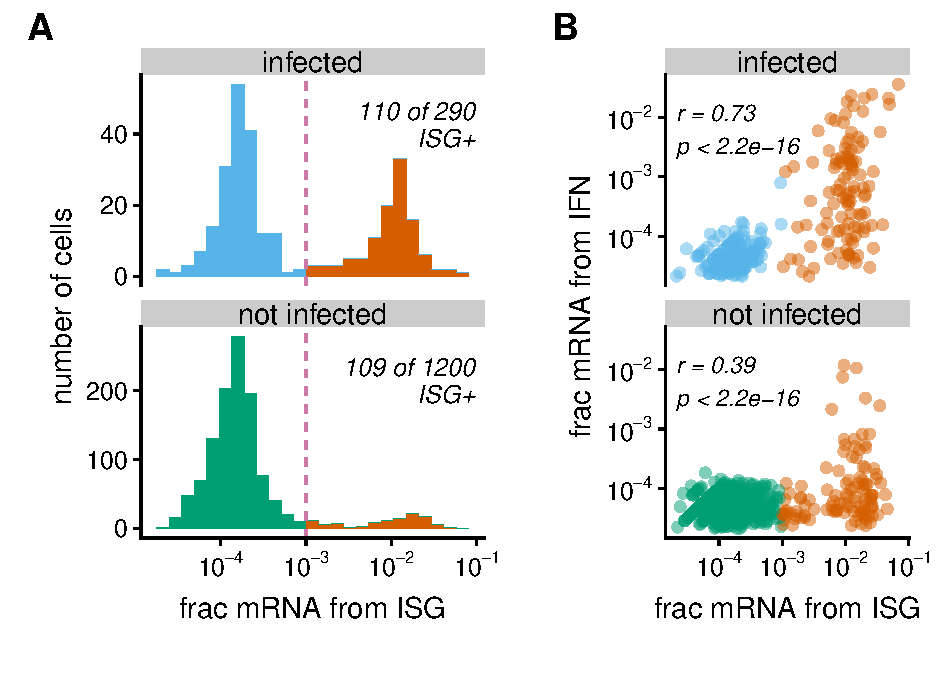
\includegraphics[width=0.8\textwidth]{figures/single_cell_figures/p_isg.pdf}}
\label{figsupp:ISG}

\figsupp[Unsupervised t-SNE clustering shows that cell-to-cell variation in influenza genes, IFN genes, and ISGs explains a substantial part of the structure of the data.]
{To generate an unbiased representation of the factors that distinguished the transcriptomes of the cells in our experiments, we used unsupervised t-SNE~\citep{maaten2008visualizing} as implemented in \texttt{Monocle}~\citep{qiu2017reversed, trapnell2014dynamics} to generate a two-dimensional representation of the data.
In the t-SNE plot, each point is a different cell and cells with similar transcriptomes are closer together.
Each panel shows the same t-SNE plot, but the cells are colored differently in each panel based on the amount of viral, IFN, or ISG mRNA shown on a log (top) or linear (bottom) scale.
As is clear from this plot, expression of influenza genes, IFN, and ISGs help explain the structure of the data, since cells with high expression of these genes clearly group together.
}
{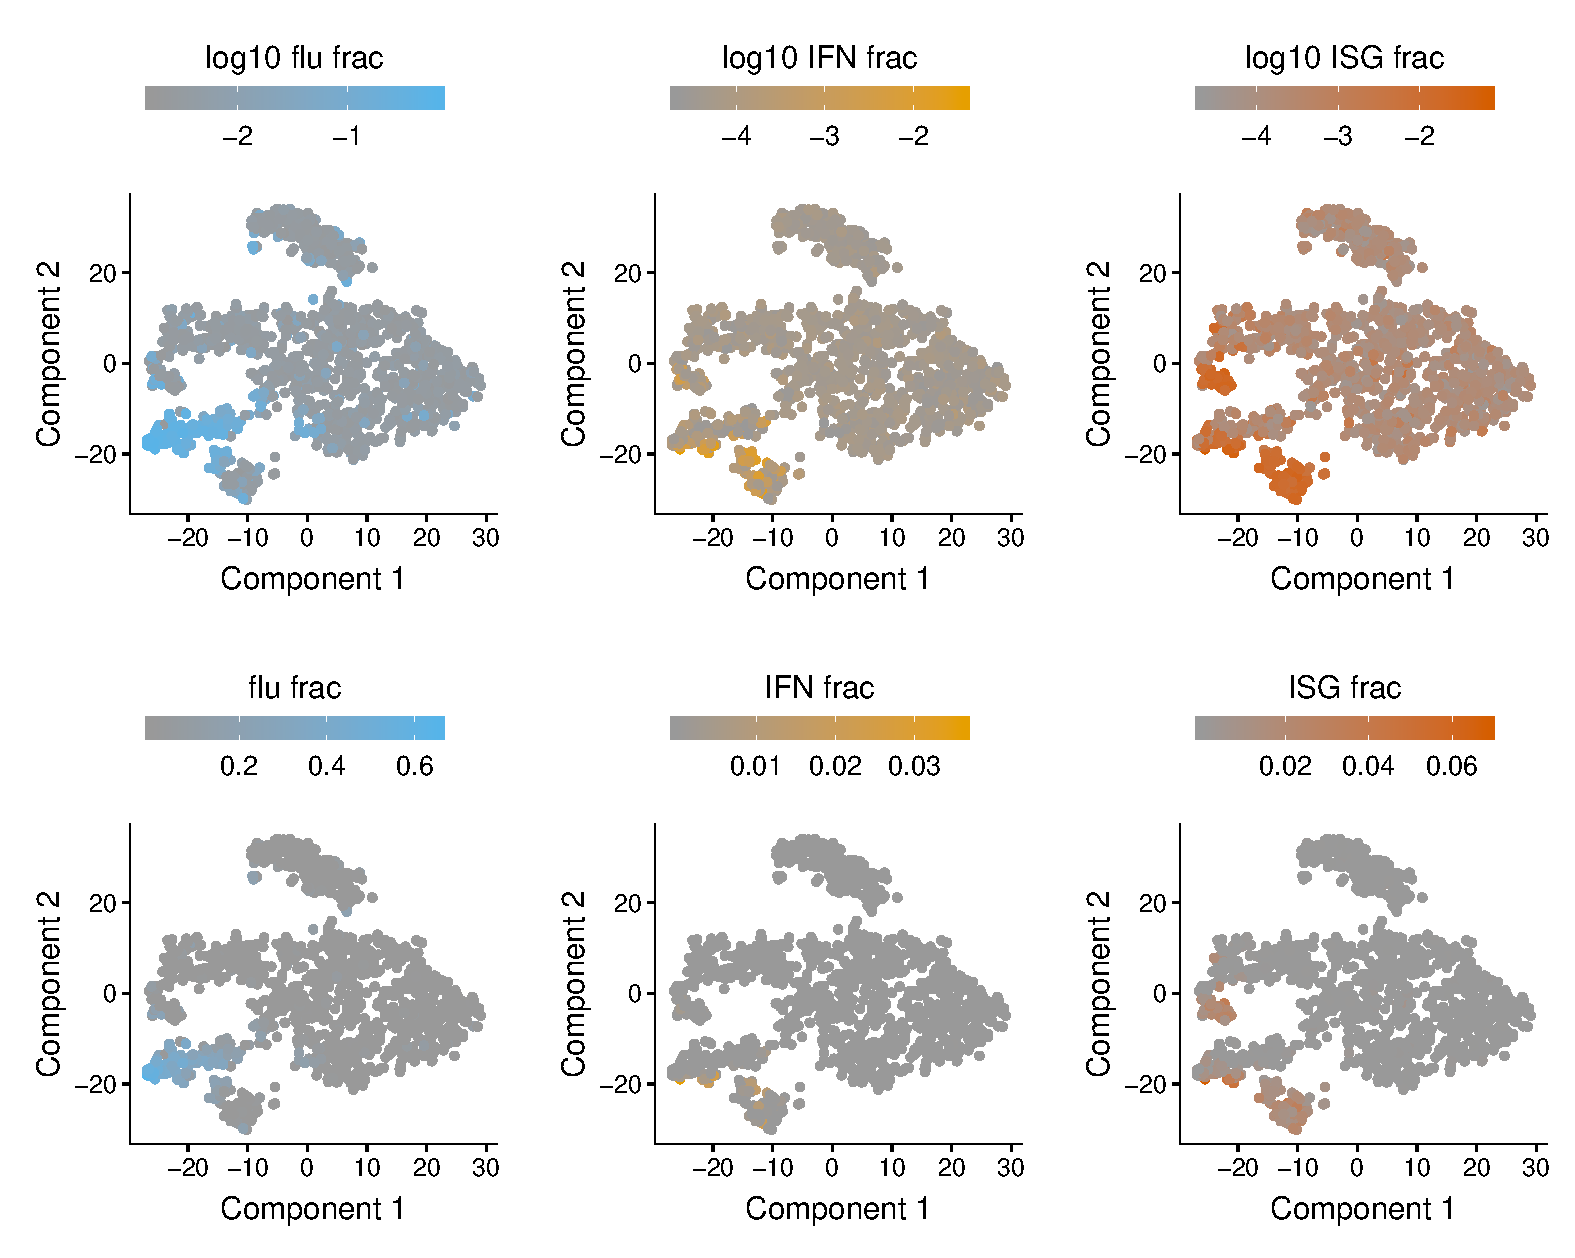
\includegraphics[width=\textwidth]{figures/single_cell_figures/p_tsne.pdf}}
\label{figsupp:tSNE}

\figdata{Genbank files giving the sequences of the wildtype and synonymously barcoded viruses are in \url{https://github.com/jbloomlab/IFNsorted_flu_single_cell/blob/master/data/flu_sequences/flu-wsn.gb} and \url{https://github.com/jbloomlab/IFNsorted_flu_single_cell/blob/master/data/flu_sequences/flu-wsn-double-syn.gb}.}
\label{figdata:virus_seqs}

\end{fullwidth}
\end{figure}
%%% end approach figure


\subsection{Viral genotypes in IFN+ and IFN- influenza-infected cells}
\FIG{genotypes} and \FIGSUPP[genotypes]{genotypes_by_ifn} and \FIGDATA[genotypes]{genotypes}


%%% start genotypes figure %%%
\begin{figure}
\begin{fullwidth}
{\centering
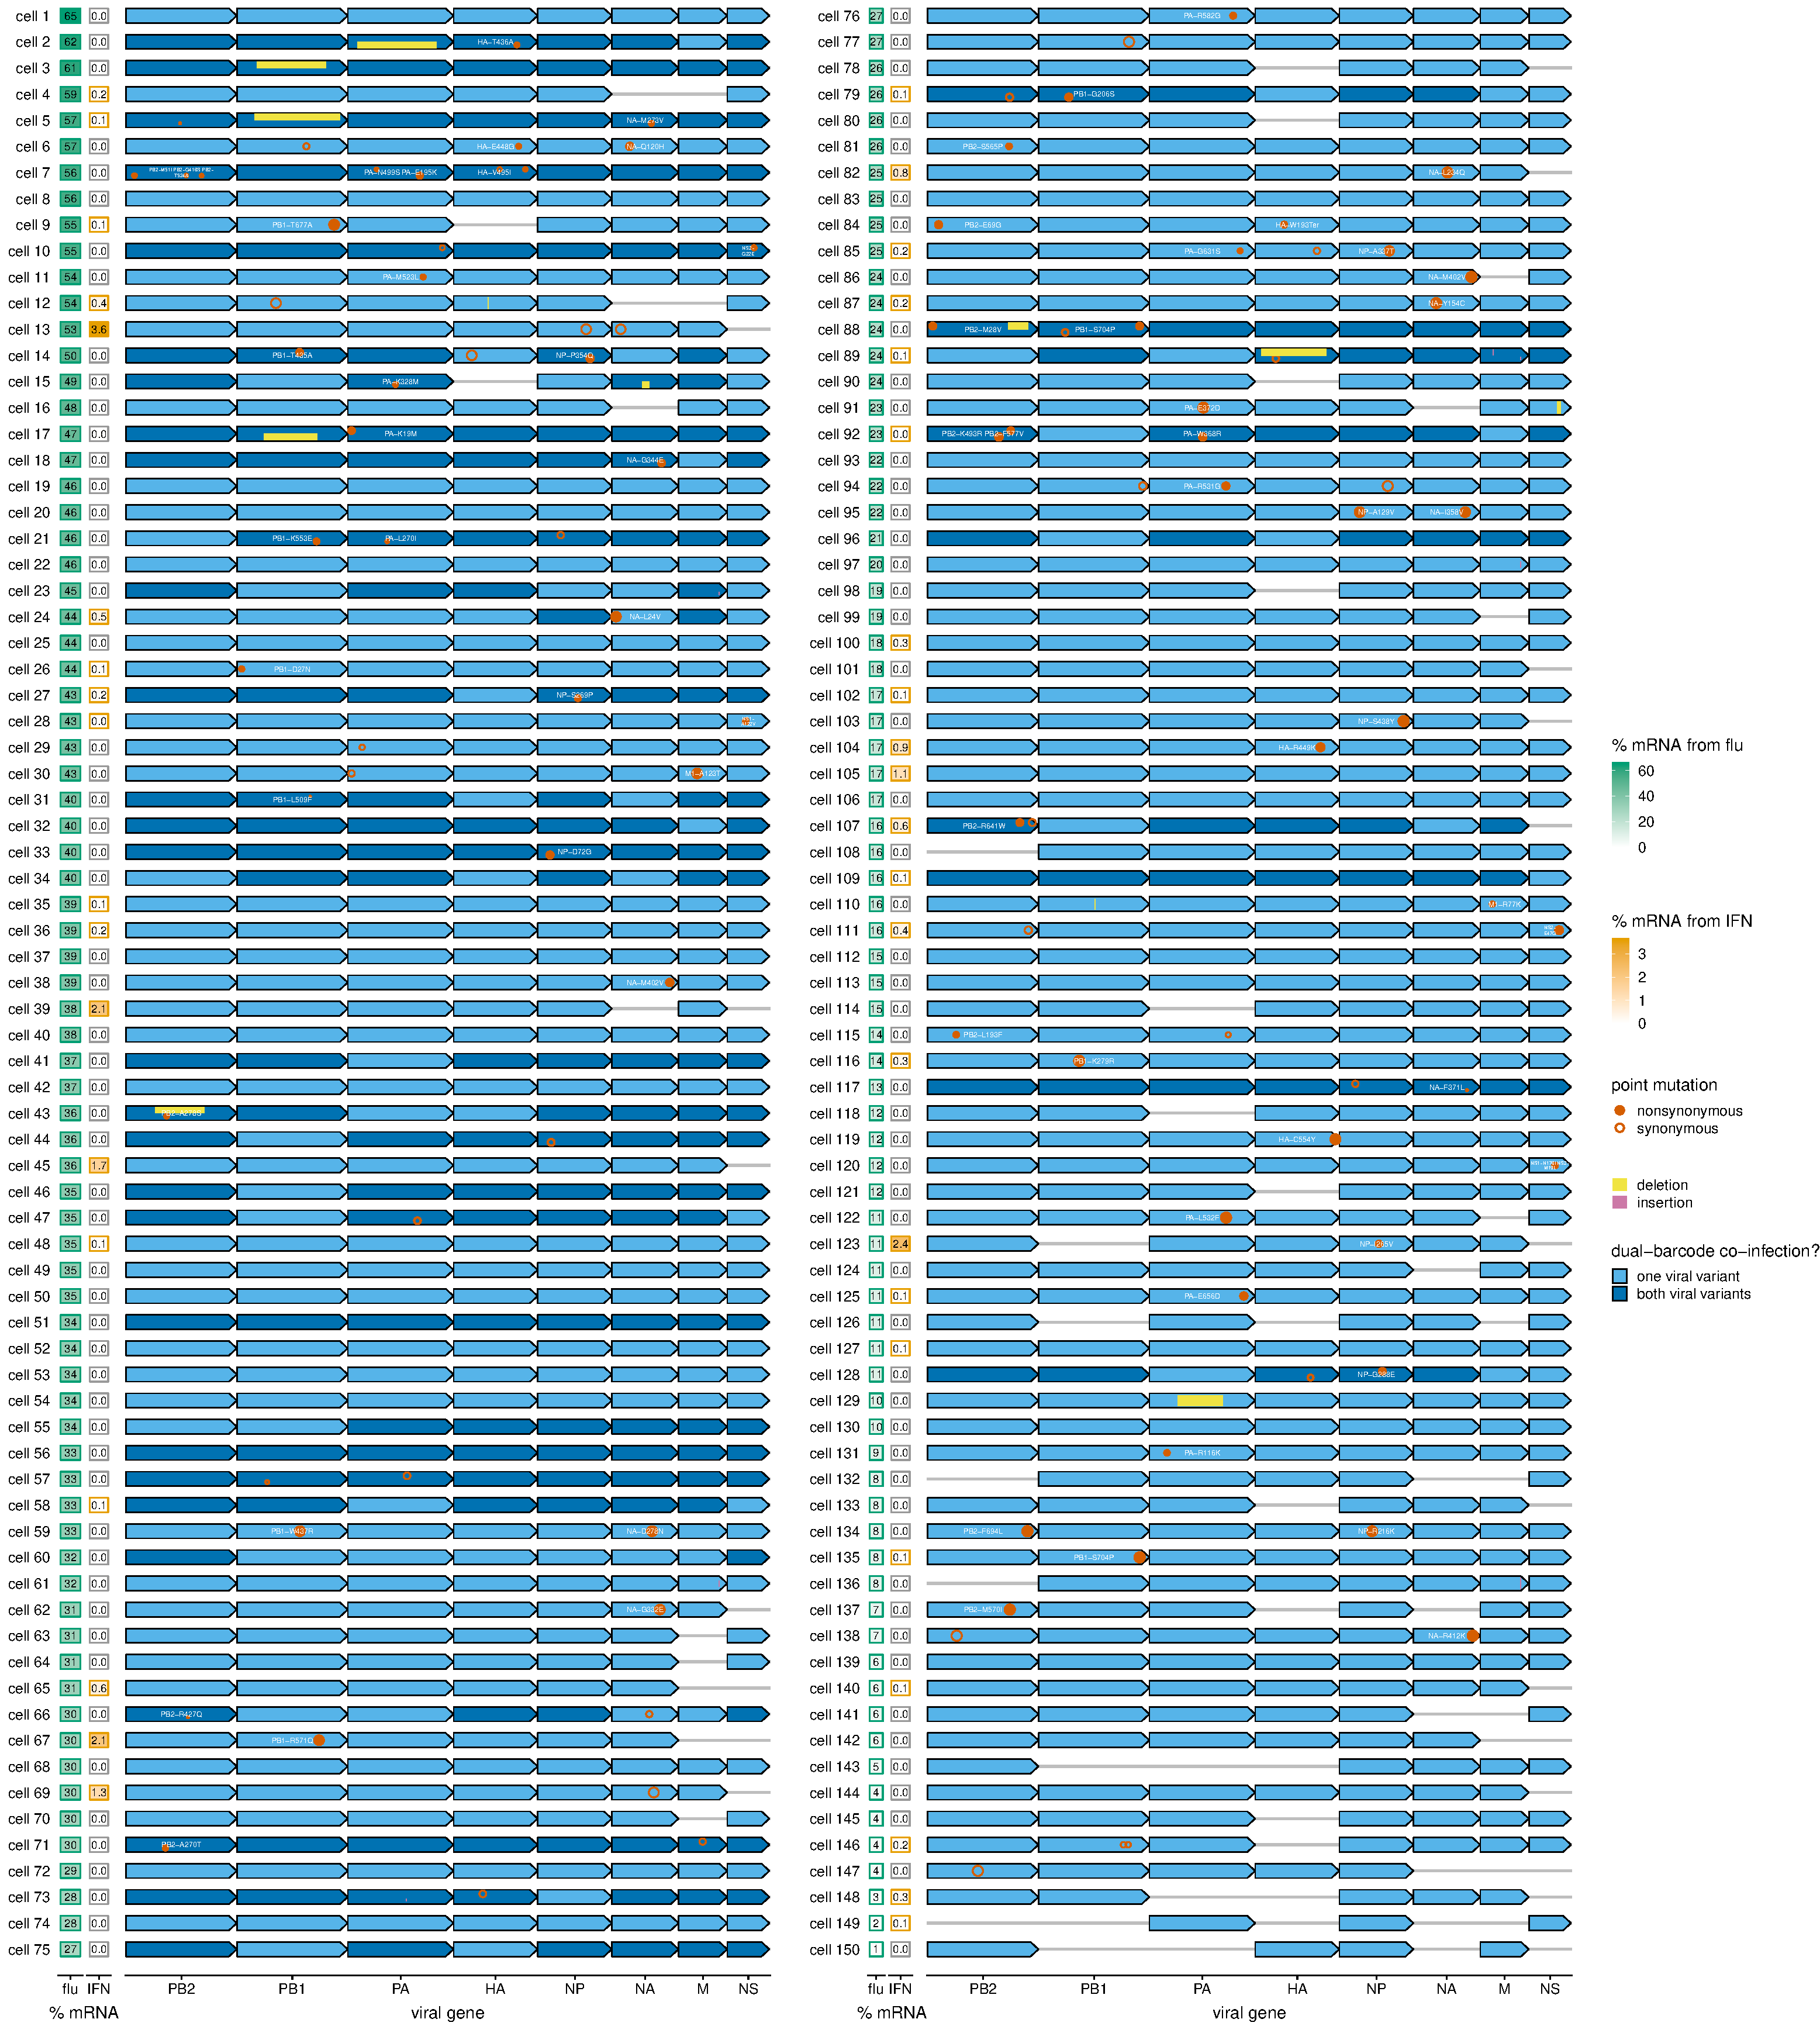
\includegraphics[height=0.8\textheight]{figures/single_cell_figures/p_genotypes.pdf}
}
\caption{
Viral genotypes and infection outcomes in single cells.
Each row shows a single infected cell.
Arrows indicate the presence of a viral gene from a single viral barcode variant (light blue) or both barcode variants (dark blue).
Circles and boxes indicate mutations or indels as described in the legend.
Circle areas and box heights are proportional to the fraction of PacBio CCSs that report the mutation (see \FIGDATA[genotypes]{genotypes} for numerical data).
For dual-barcode infections, mutations / indels for the wildtype viral variant are on the top half of the arrow and those for the synonymously barcoded variant are on the bottom half. 
Green boxes to the left show the percent of all mRNA in that cell derived from virus.
Orange boxes show the percent of cellular mRNA derived from IFN, with boxes framed in orange indicating cells classified as IFN+ in \FIG{experiment}H.
}
\label{fig:genotypes}

\figsupp[Strategy for detecting strand exchange during sequencing of full-length viral genes.]
{The library preparation for PacBio sequencing of the cDNA for the full-length viral genes requires many cycles of PCR in order to produce a sufficient amount of DNA for sequencing.
A major concern is whether strand exchange during this PCR could scramble mutations and 10X cell barcodes / UMIs from different molecules.
We can detect PCR strand exchange by leveraging the fact that our cells were infected with a mix of wildtype virus and virus carrying synonymous barcodes near both termini of each gene.
If there is no strand exchange, all molecules should either be wildtype or have the synonymous mutations at the viral barcode sites.
But strand exchange will create some molecules that have a mix of wildtype nucleotides in the viral barcode at one termini and synonymous mutations in the viral barcode at the other termini.
\FIGSUPP[genotypes]{CCSs} shows the frequencies with which these different types of molecules were observed during the PacBio sequencing.
Note that since the rate of homologous recombination in influenza virus in negligible~\citep{boni2008homologous}, such mixed-barcode molecules are \emph{not} expected to be generated naturally during co-infection.
}
{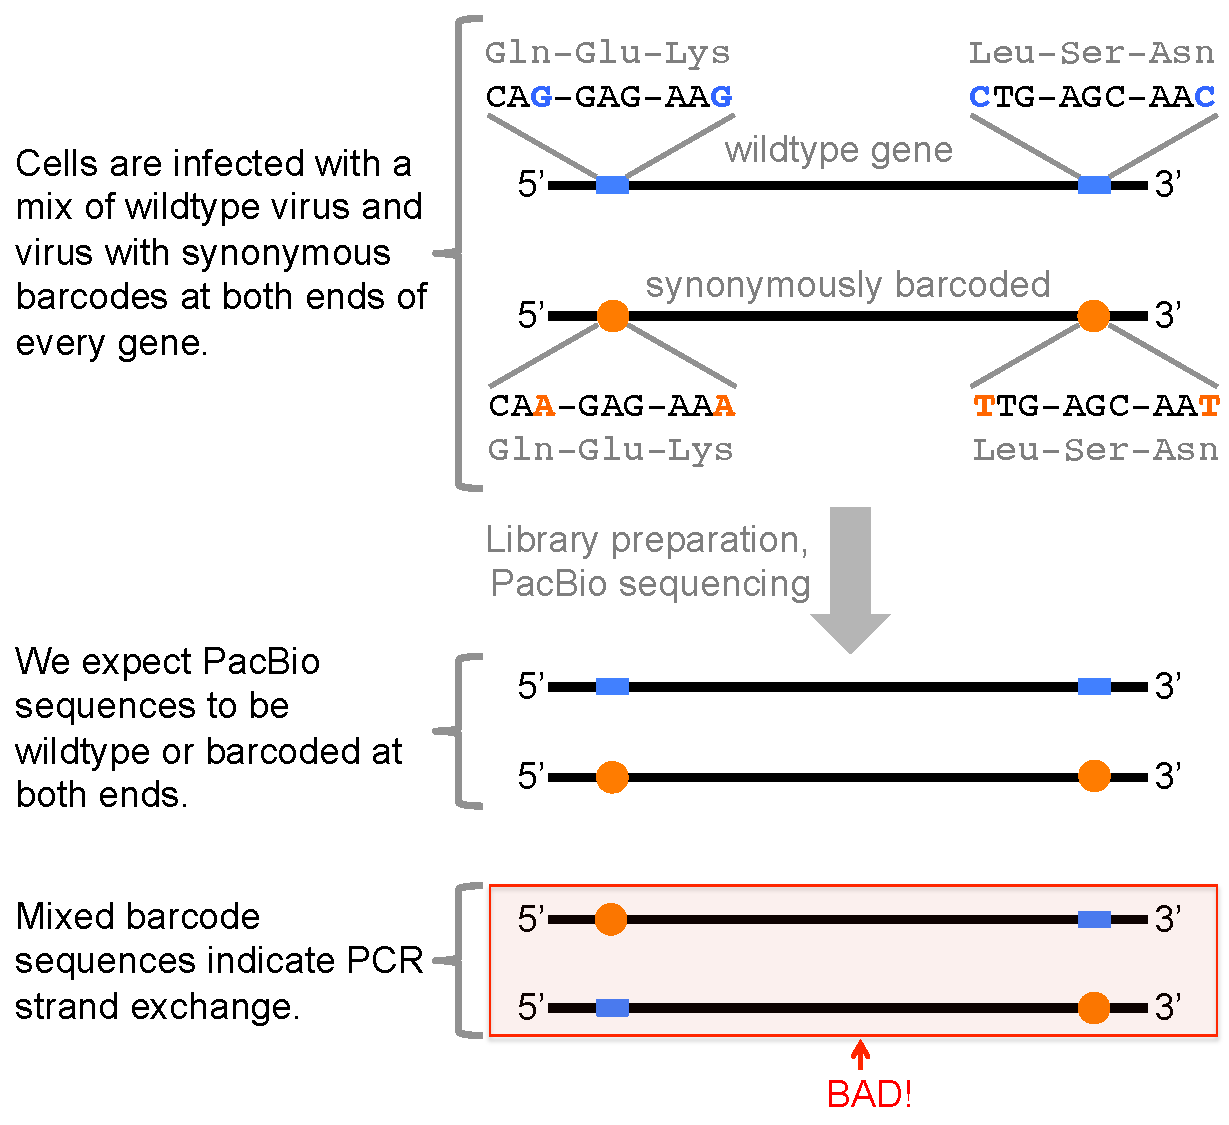
\includegraphics[width=0.6\textwidth]{figures/StrandExchangeSchematic/StrandExchangeSchematic.pdf}}
\label{figsupp:StrandExchange}

\figsupp[Number of PacBio circular consensus sequences and PCR strand exchange rate.]
{
The number of PacBio CCSs that passed quality-control steps and aligned to an influenza virus gene.
Note that these sequences were obtained using several PacBio runs, some of which were loaded with different amounts of the various viral genes in order to increase coverage on genes that were needed in order to obtain the full sequences of virions infecting cells.
Therefore, unlike the 10X transcript count data in \FIG{experiment}H, the numbers of CCSs for different genes should \emph{not} be taken as an indicator of their abundance in the infected cells.
Especially for the polymerase genes (PB2, PB1, and PA), many of the CCSs corresponded to genes with internal deletions, since these shorter forms of the genes were presumably preferentially amplified during PCR.
Therefore, the plot is faceted by the number of CCSs for any length of the gene, and for full-length genes.
Note that the disproportionate sequencing of the shorter internally deleted genes should not greatly affect the genotype calling in \FIG{genotypes} since UMIs were used to collapse duplicate sequences for the same gene, and cell barcodes to collapse duplicate sequences from the same cell.
The bars are colored by whether the sequence can be identified as being derived from the wildtype viral variant, the synonymously barcoded variant, or represents a mixed barcode molecule (see \FIGSUPP[genotypes]{StrandExchange}).
From the frequencies of these different forms, we estimate~\citep{bloom2018estimating} that 5.7\% of molecules are chimeric due to PCR strand exchange.
Note that about half of these PCR chimeras could be identified by the presence of mixed viral barcodes and removed from subsequent analyses, leaving $\sim$3\% un-identified chimeras.
Note also that for some molecules (mostly polymerase genes with internal deletions) one of the barcode sites was deleted from the molecule and so the barcode identity could only be partially called.
A negligible number of molecules have low-accuracy sequence or unexpected nucleotide identities at the sites of the viral barcode.
}
{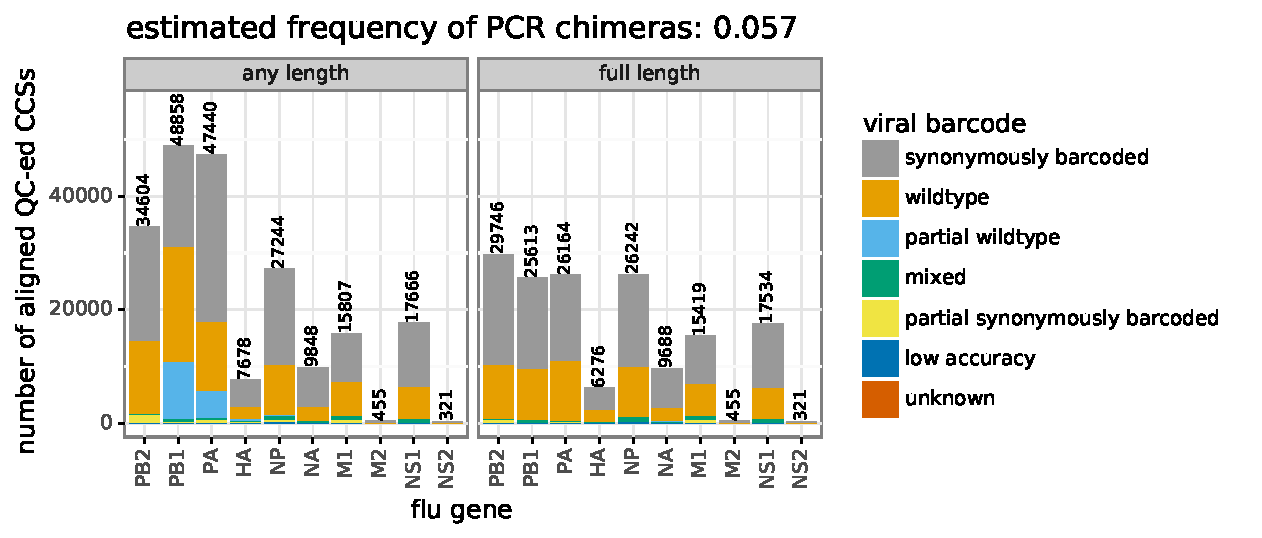
\includegraphics[width=\textwidth]{figures/pacbio_single_cell_figures/ccs_per_viralbarcode.pdf}}
\label{figsupp:CCSs}

\figsupp[Number of cells for which genotype(s) of infecting viruses were completely determined.]
{Cells for which we could determine the full sequences of all genes expressed by the infecting virus(es).
{\bf (A)} We could call the complete genotypes of the infecting virus(es) for the majority of cells infected with just a single viral barcode variant, but only a minority of cells co-infected with both viral barcodes.
{\bf (B)} The cells for which we could call complete viral genotypes tended to have higher expression of viral mRNAs than cells for which we could not call complete genotypes.
This makes sense, as cells with more viral mRNA are more likely to have their viral genes captured in the PacBio sequencing, which is only able to capture a small fraction of the total transcripts identified by the 3'-sequencing of the 10X platform.
The lower calling rate for dual-barcode co-infections relative to single barcode infectionis is probably because these co-infections have more viral genes that must be sequenced (potentially a copy of each viral gene from each viral variant), increasing the chances that one of these genes is missed by the PacBio sequencing. 
An important implication of this plot is that the cells for which we call complete viral genotypes are \emph{not} a random subsampling of all infected cells in the experiment, but are rather enriched for cells that have high levels of viral mRNA and do not have dual-barcode viral infections.
Note also that this plot is limited to the cells that were called as infected (\FIG{experiment}D) and could clearly be classified as IFN- or IFN+ (\FIG{experiment}H).
}
{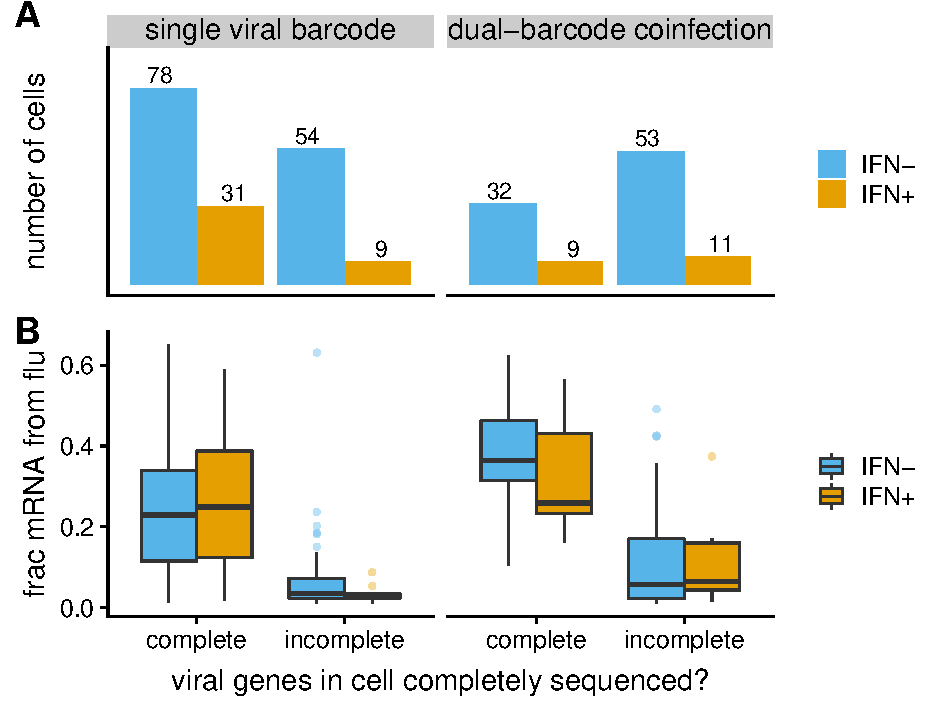
\includegraphics[width=0.8\textwidth]{figures/single_cell_figures/p_cells_complete.pdf}}
\label{figsupp:ncells}

\figsupp[Genotypes and infection outcomes plotted separately for IFN+ and IFN- cells.]
{This plot shows the same data as \FIG{genotypes}, but with cells separated into columns based on whether they are IFN- (left column) or IFN+ (right column).}
{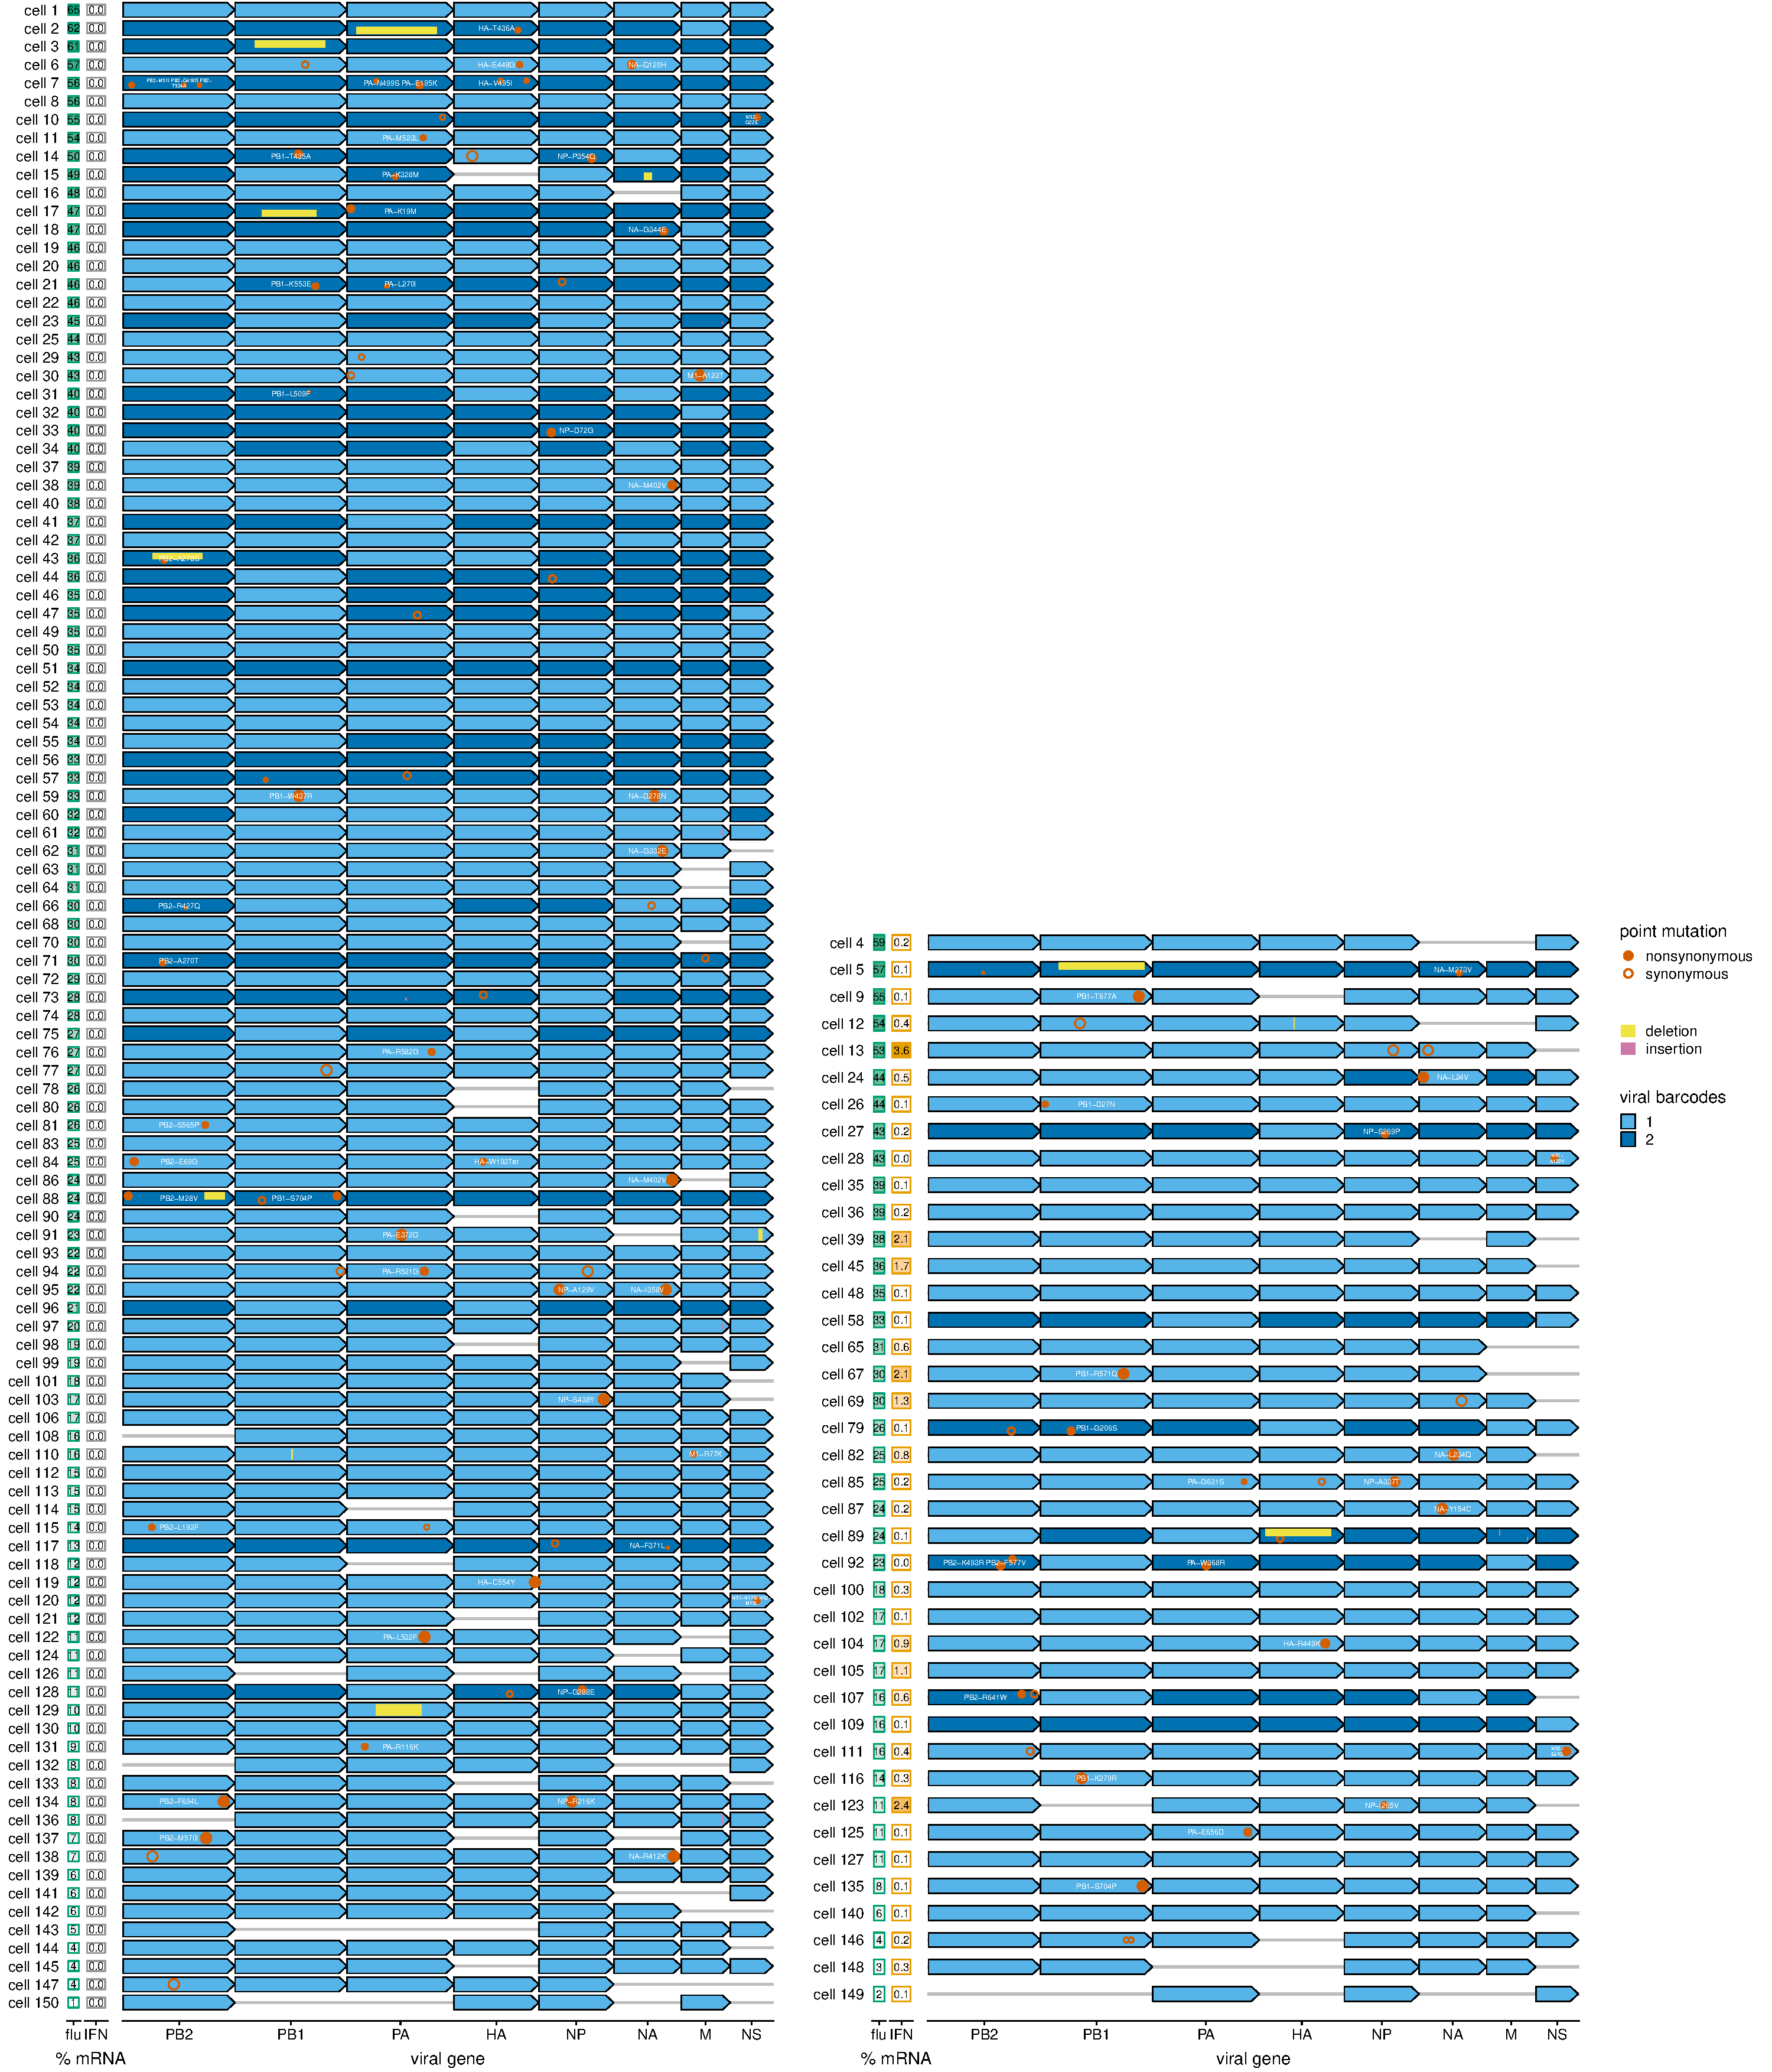
\includegraphics[width=\textwidth]{figures/single_cell_figures/p_genotypes_by_ifn.pdf}}
\label{figsupp:genotypes_by_ifn}

\figdata{A CSV file giving the genotypes is at \url{https://github.com/jbloomlab/IFNsorted_flu_single_cell/blob/master/paper/figures/single_cell_figures/genotypes.csv}.}
\label{figdata:genotypes}

\end{fullwidth}
\end{figure}
%%% end genotypes figure %%%




%%% begin mutations figure %%%
\begin{figure}
\begin{fullwidth}
{\centering
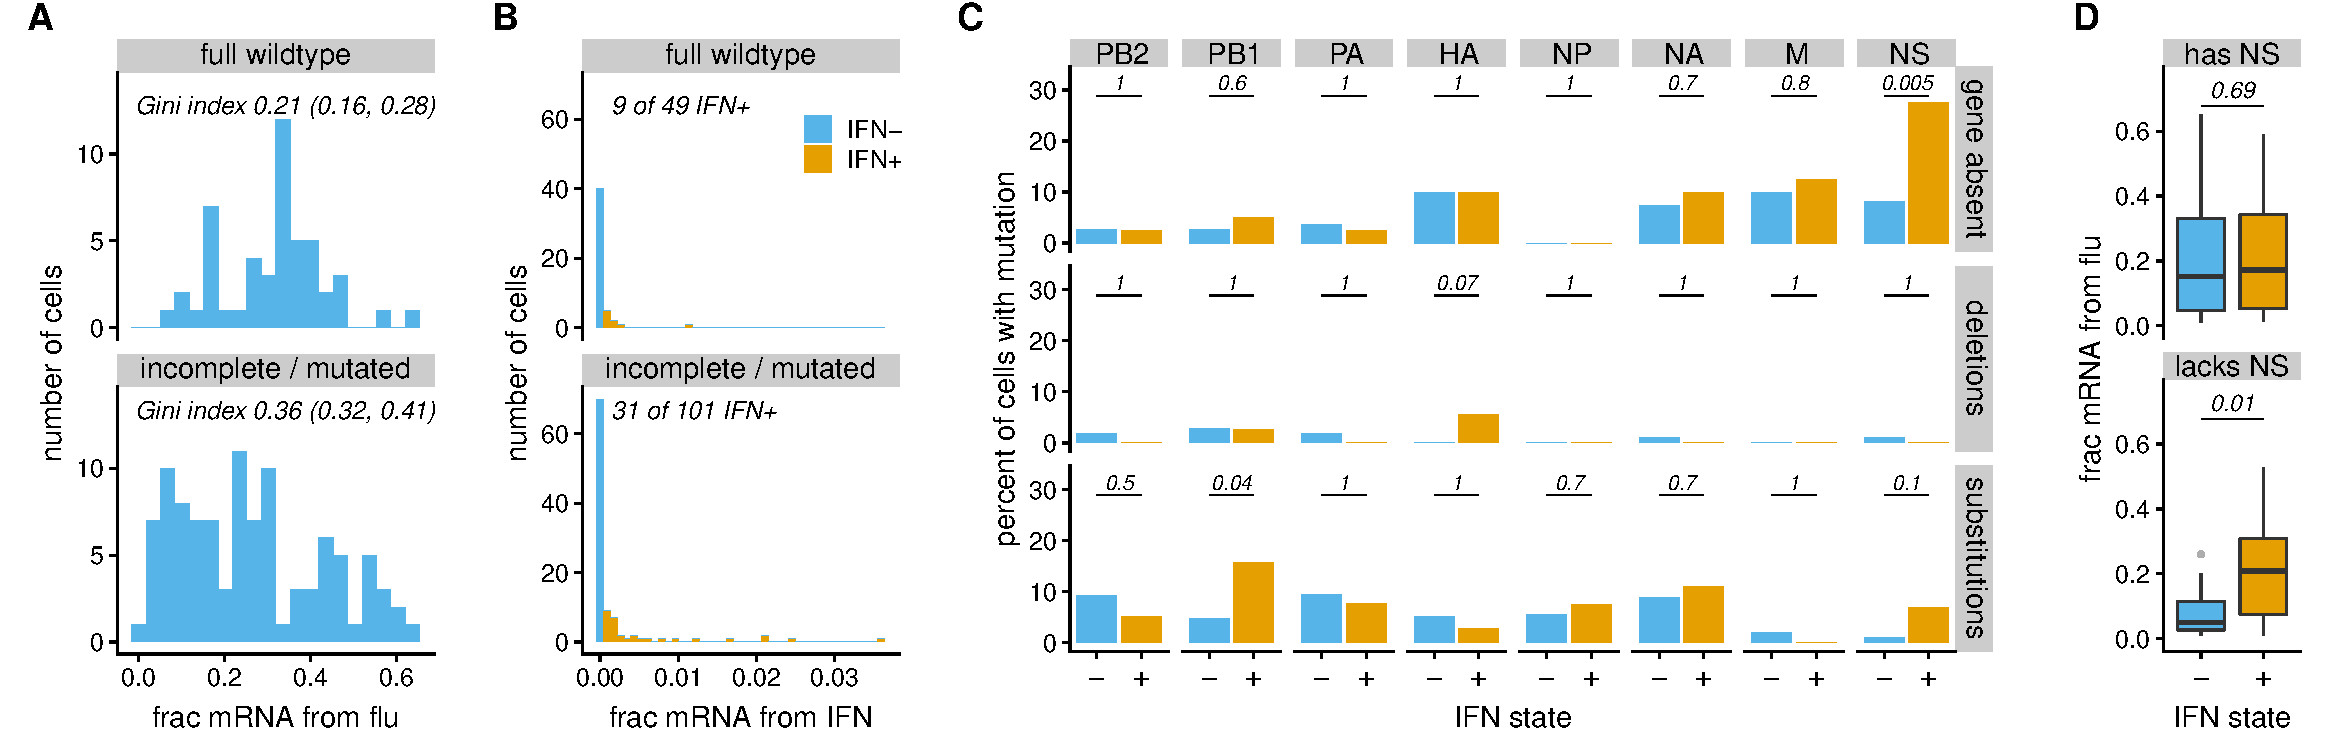
\includegraphics[width=\linewidth]{figures/single_cell_figures/p_mutations.pdf}
}
\caption{
Viral genetic variation partially explains the heterogeneity in viral burden and IFN induction among the infected cells for which we sequenced all expressed viral genes (\FIG{genotypes}).
{\bf (A)} 
The percent of all mRNA derived from virus, faceted by whether the cells express wildtype copies of all eight viral genes, or fail to express a wildtype copy of one or more genes (due to gene absence, amino-acid substitution, insertion, or deletion).
Cells infected by full wildtype virus exhibit less heterogeneity in viral burden as quantified by the Gini index (95\% confidence intervals are indicated).
{\bf (B)}
There is a trend for cells infected by full wildtype virus to express less IFN.
{\bf (C)}
Some specific forms of viral genetic variation are associated with IFN induction.
The top panel show the percent of IFN+ and IFN- cells that fail to express each viral gene.
The middle and bottom panels show the percent of IFN- and IFN+ cells that have a deletion or amino-acid substitution in each viral gene, conditioned on the cell expressing that gene.
Numbers above the bars give P-values (Fisher's exact test) and associated Q-values~\citep{storey2003statistical} for rejecting the null hypothesis that percents are equal among IFN- and IFN+ cells. 
Absence of NS is strongly associated with IFN induction, and amino-acid substitutions in PB1 or NS and deletions in HA are weakly associated with IFN induction.
Only the absence of NS remains significant at a false-discovery rate of 10\%.
\FIGSUPP[mutations]{allcells} shows that the trends remain largely the same if we also analyze infected cells with incomplete viral sequence information, with the addition of a trend towards IFN induction associated with \emph{presence} of PB2 and PA. 
\FIGSUPP[mutations]{isg} shows that the trends also remain largely similar if we analyze the association of viral genetic variation with ISG expression rather than IFN expression.
Insertions are not shown as a mutation type as they are extremely rare (\FIG{genotypes}).
{\bf (D)}
There is no association between IFN induction and the amount of viral mRNA in cells that express NS, but viral burden is associated with IFN induction among cells that lack NS.
Note that throughout this figure, we only consider as substitution mutations that are non-synonymous.
}
\label{fig:mutations}

\figsupp[Analysis as in \FIG{mutations}C but including infected cells with incomplete viral sequence information.]
{This plot differs from \FIG{mutations}C in that it also includes data from cells for which some viral genes were not fully sequenced.
For incompletely sequenced cells, deletions and substitutions are included in the counts when that particular viral gene is sequenced.
The major trends in \FIG{mutations}C are also true for the larger dataset in this figure.
In addition, there is now a modest trend for infected cells that fail to express PB2 and PA \emph{not} to express IFN.
}
{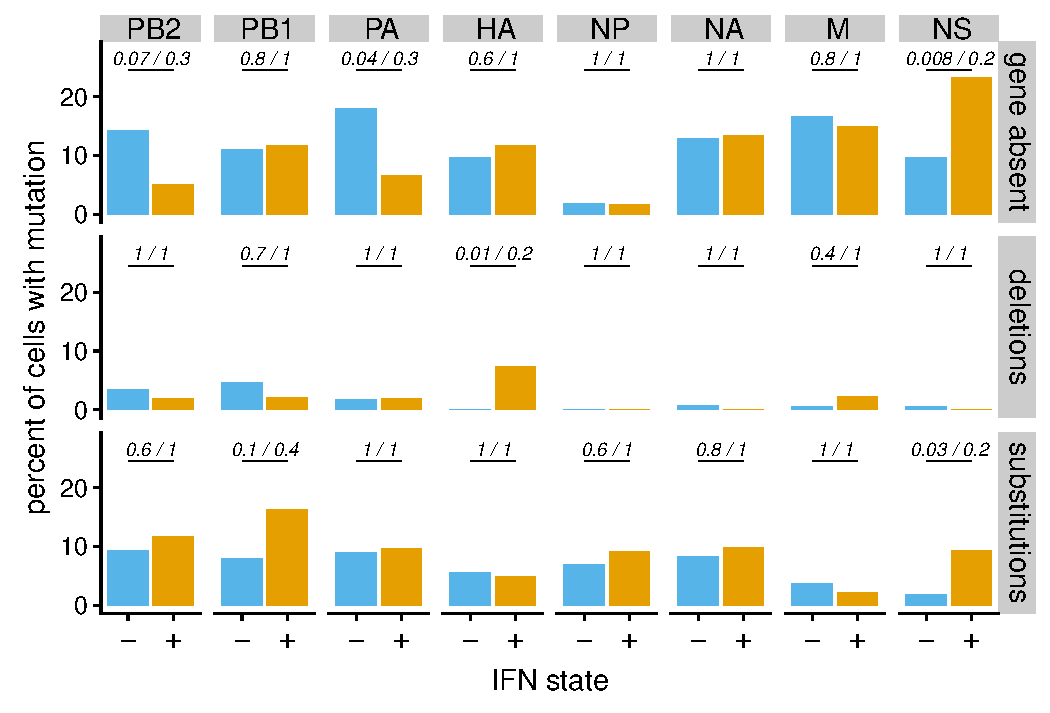
\includegraphics[width=\textwidth]{figures/single_cell_figures/p_muts_ifn_all.pdf}}
\label{figsupp:allcells}

\figsupp[Association of viral genetic variation and ISG expression.]
{This plot shows the same information as panels \FIG{mutations}B-D except that it shows the association of viral gene absence / mutations with ISG expression rather than IFN expression.
Cells are classified as ISG+ or ISG- as in \FIGSUPP[experiment]{ISG}.
The major viral features that associate with IFN induction also associate with ISG expression.
Specifically, cells that express wildtype copies of all eight viral genes tend to express ISGs less frequently and at lower levels
The absence of NS is strongly associated with higher ISG expression.
Viral burden is not associated with ISG expression levels in NS-sufficient infections, but is in NS-deficient infections.
}
{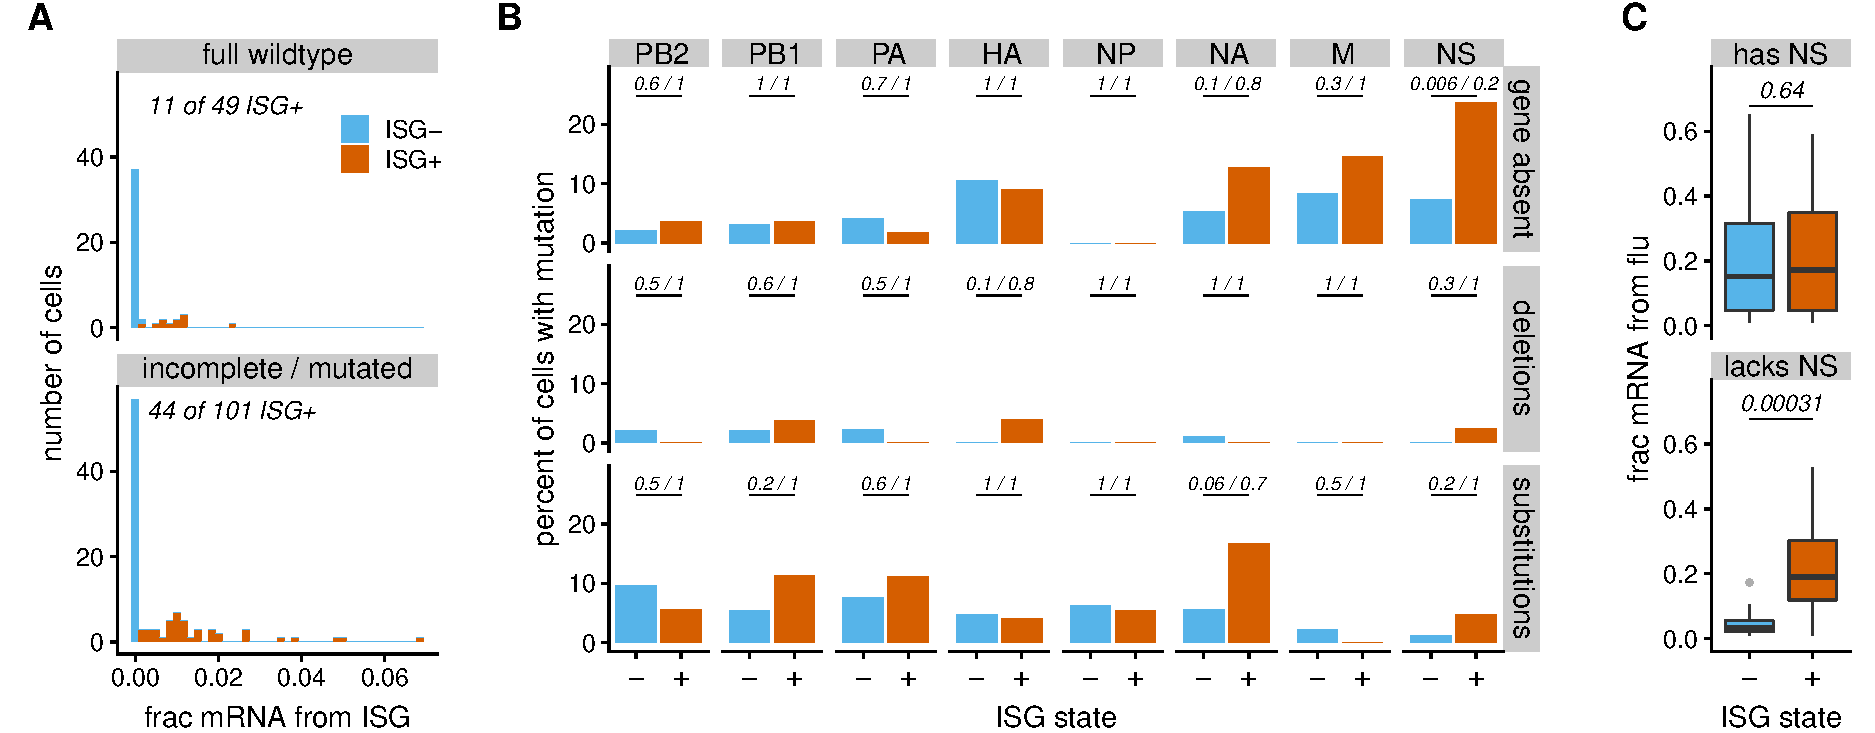
\includegraphics[width=\textwidth]{figures/single_cell_figures/p_mutations_isg.pdf}}
\label{figsupp:isg}

\figdata{A CSV file giving the viral mutations and related information in \FIG{mutations} is at \url{https://github.com/jbloomlab/IFNsorted_flu_single_cell/blob/master/paper/figures/single_cell_figures/mutations.csv}.}
\label{figdata:mutations}

\end{fullwidth}
\end{figure}
%%% end mutations figure %%%

\section{Discussion}

Add text

\section{Methods and Materials}

\subsection{IFN reporter cell lines}
\jdbcomment{Alistair writes this}
For our type I interferon reporters, A 1kb region upstream of the human IFNB1 gene was cloned into the pHAGE2 lentiviral vector, with a NotI site immediately downstream serving as an artificial Kozak sequence (REF). 
Downstream of this NotI site, each of the following reporter constructs was cloned: mCherry, mNeongreen, and mNeongreen translationally linked to low-affinity nerve growth factor lacking the C-terminal signaling domain (LNGFR$\Delta$C) by a p2A linker (REFS).
For our type III interferon reporters, a 1.2kb region upstream of the human IL29 (IFNL1) gene was cloned into the pHAGE2 vector, with the native kozak sequence left at the 3' end. 
Downstream of this promoter zsGreen translationally linked to LNGFR$\Delta$C via a p2A linker was cloned. 
Replication-incompetent lentivirus was generated from these vectors as previously described (REF).
A monolayer of A549 cells in D10 was transduced with each lentivirus in the presence of 5 $\mu$g polybrene, and sorted as single cells. 
These single cell clones were grown and tested for reporter activity by poly I:C transfection---a potent agonist of the RIG-I pathway.
Critically, cells propagated and used in experiments were not exposed to poly I:C,  thus avoiding selection on survival post interferon-induction.
For our dual- type I and type III reporter, a single-cell clone of our type III reporter strain was transduced with our type I reporter bearing the mCherry fluorescent marker and subsequently propagated as a single cell clone and validated as above.

Reporter sequences \FIGDATA[IFNrare]{reporter_sequences}



\subsection{Viral stocks}
\jdbcomment{Alistair writes this}
All viruses were generated using reverse-genetics as previously described.
All infections were performed in influenza growth media as previously described.
Briefly, bidirectional plasmids producing viral mRNA and vRNA are transfected into a co-culture of MDCK-SIAT1 and 293t cells grown in D10.
After 24h, media is changed from D10 to influenza growth media.
Between 48h and 72h post-infection, depending on viral growth kinetics, supernatant was harvested and titered by TCID50.
Virus was subsequently expanded on MDCK-SIAT1 cells as described below.
For all viral variants, the described mutations were introduced into reverse-genetics plasmids using PCR mutagenesis. 
For the HA-flanked mCherry pseudovirus, a plasmid was generated similarly to a previously-described HA-flanked eGFP vector.
Synonymously-barcoded virus utilized previously described 3' synonymous mutations, and two newly-introduced single-nucleotide synonymous mutations at the 5' end of each viral gene.
Wild-type, synonymously-barcoded, NS1-inactivated, and single-nucleotide variant viruses were all grown in unmodified MDCK-SIAT1 and 293t cells.
Viral variants bearing large internal deleltions in the PB1 segment were grown in MDCK-SIAT1 and 293t cells expressing PB1 as previously described.
Pseudovirus expressing mCherry in place of eGFP was grown in MDCK-SIAT1 and 293t cells expressing HA as previously described.

Wildtype and synonymously barcoded viruses in \FIGDATA[experiment]{virus_seqs} obtained from reverse-genetic transfections was subsequently propagated at an MOI of 0.001 for 72h twice in MDCK-SIAT1 cells (wild-type) or once at an MOI of 0.01 (barcoded) for 60h in order to generate potential immunostimulatory diversity.
For analyses of interferon induction, an additional wild-type stock of virus was grown at an MOI of 0.01 for 36h in order to generate a population relatively free of defective particles. (WILL REPEAT WITH 48H STOCK AS DESCRIBED BELOW)
Viruses bearing SNPs, deletions in PB1, NS1-inactivation mutations, and HA-mCherry pseudovirus were all propagated at an MOI of 0.01 for 48h owing to slower growth kinetics. 
All stocks were subsequently titered by TCID50, using complementing cells where necessary.
Additionally, for qPCR experiments, stocks were titered by qPCR against the viral HA segment using a plasmid standard to determine relative genome copy numbers between viral stocks.


\subsection{Single-cell infections and transcriptomics using 10X Chromium on IFN-enriched cells}
Type I interferon reporter A549 cells (mNeongreen-p2A-LNGFR$/Delta$C) were infected with a mixture of barcoded (MOI 0.1) and wild-type (MOI 0.02) virus. 
These differing MOI's were chosen to roughly match the fraction of HA-positive cells in flow cytometry experiments (and thus biologically active particles) titering these two stocks. 
Infections were allowed to proceed for 12h.
Cells were trypsonized, trypsin was quenched with D10 media, and cells were resuspended in de-gassed PBS supplemented with 0.5\% bovine serum albumin and 5 mM EDTA. 
Cells were then incubated with anti-LNGFR MACSelect Microbeads and passed over an MS magnetic column twice, selecting the positive population each time. The original, unsorted, population was then added back in to approximately 10 percent of the final cell fraction in order to ensure the presence of interferon negative cells. 
At this point, uninfected MDCK-SIAT1 cells were also added to approximately 10 percent of the final cell fraction for doublet and lysis metrics. 
The final cell suspension was counted using a disposable hemocytometer and loaded on the 10x Genomics instrument at a targeted capture of ~1500 cells. 

This sample was then processed according to the manufacturer's protocol using the Chromium Single Cell 3? Library and Gel Bead Kit v2 with one important modification; rather than process all full-length cDNA through enzymatic fragmentation, several nanograms were retained for targeted sequencing as described below.


\jdbcomment{Alistair writes this}

\subsection{Enrichment and preparation of viral cDNA for PacBio sequencing}
Approximately 1ng of full-length 10x-barcoded cDNA was used as template in an emulsion PCR using the 


\jdbcomment{Alistair writes this}

\subsection{Computational analysis of single-cell transcriptomic and viral sequence data}
A computational pipeline that performs all steps in the data analysis is available at \url{https://github.com/jbloomlab/IFNsorted_flu_single_cell}~\citep{russell2018github}. 
This pipeline is orchestrated by \texttt{Snakemake}~\citep{koster2012snakemake}, and begins with the raw sequencing data and ends by generating the figures shown in this paper.
The sequencing data and annotated cell-gene matrix are available on the GEO repository under \jdbcomment{add accession}.

Briefly, the raw deep sequencing data from the Illumina 3'-end sequencing were processed using the 10X Genomics software package \texttt{cellranger} (version 2.2.0). 
We built a multi-species alignment reference consisting of a concatenation of the human and influenza virus transcriptomes (the first ``species'') and the canine transcriptome (the second ``species''). 
The human transcriptome was generated by filtering genome assembly GRCh38 for protein-coding genes defined in GTF file GRCh38.87.
The influenza virus transcriptome consisted of the mRNAs for the wildtype A/WSN/1933 virus strain in \FIGDATA[experiment]{virus_seqs} (the \texttt{cellranger} alignment is sufficiently permissive that it aligns sequences from both the wildtype and synonymously barcoded viral variants to this transcriptome).
The canine transcriptome was generated by filtering genome assembly CanFam3.1 for protein-coding genes defined in GTF file CanFam3.1.87.
The \texttt{cellranger} software was used to align the Illumina 3'-end sequencing reads to this multi-species transcriptome, call human+influenza and canine cells (\FIG{experiment}B), and generate a matrix giving the expression of each gene in each single cell.
We used a custom Python script to determine the number of influenza virus reads that could be assigned to the wildtype or synonymously barcoded virus, and added this information to the annotated the cell-gene matrix.

The PacBio sequences of the full-length viral genes were analyzed as follows.
First, we used version 3.1.0 of PacBio's \texttt{ccs} program (\url{https://github.com/PacificBiosciences/unanimity}) to build circular consensus sequences (CCSs) from the subreads files, requiring at least 3 passes and a minimum accuracy of 0.999.
We further processed these CCSs using custom Python code and the \texttt{minimap2}~\citep{li2018minimap2} long-read aligner (version 2.11-r797).
The Python code has been implemented in the API of \texttt{dms\_tools2}~\citep[][\url{https://jbloomlab.github.io/dms_tools2/}]{bloom2015software} package (version 2.3.0).
A Jupyter notebook that performs these analyses is at \url{https://github.com/jbloomlab/IFNsorted_flu_single_cell/blob/master/pacbio_analysis.ipynb}, and is also provided in HTML form as Supplementary~file~\ref{suppfile:pacbio_analysis}.
We refer the reader to this notebook for a detailed description and extensive plots showing the results at each step.
Here is a brief summary: we filtered for CCSs that had the expected 5' termini (from the influenza-specific primers) and 3' termini (corresponding to the 10X adaptor), and for which we could identify the cell barcode, UMI, and polyA tail.
We aligned the cDNAs flanked by these termini to the influenza transcriptome, and performed a variety of quality control steps.
At this point, we examined whether cDNAs had the synonymous viral barcodes at both ends or neither end as expected in the absence of strand exchange (\FIGSUPP[genotypes]{StrandExchange}), and reassuringly found that strand exchange was rare (\FIGSUPP[genotypes]{CCSs}).
The small number of CCSs with identifiable strand exchange were filtered from further analysis.
We then further filtered for CCSs that contained valid cell barcodes as identified by the \texttt{cellranger} pipeline, and kept just one CCS per UMI (preferentially retaining high-quality CCSs that aligned to full-length cDNAs).
Finally, we used the CCSs to call the sequence of the viral gene in each cell, calling mutations separately for each viral barcode variant.
We called mutations (insertions, deletions, and substitutions) in the viral gene sequences as follows:
\begin{enumerate}
\item Mutations with accuracies less than 0.999 (which constitute $<$0.5\% of all mutations) were ignored.
\item If all CCSs for a particular viral-barcode variant of a gene in a cell were wildtype, it was called as wildtype.
\item If any CCSs for a particular viral-barcode variant of gene in a cell had a mutation, then require at least two CCSs to call the sequence.
\item If at least two and $>$30\% of the CCSs had a specific mutation, then call that mutation as present and note its frequency among the CCSs. The exception was single-nucleotide indels in homopolymers, for which we required three CCSs to call a mutation (the reason is that the main mode of PacBio sequencing errors is short indels in homopolymers).
\end{enumerate}
The plots in \url{https://github.com/jbloomlab/IFNsorted_flu_single_cell/blob/master/pacbio_analysis.ipynb} or Supplementary~file~\ref{suppfile:pacbio_analysis} indicate that these are reasonable mutation-calling criteria.
We could call the sequences of all expressed viral genes in about half of the infected cells (\FIGSUPP[genotypes]{ncells}).
The mutations called using this pipeline are shown in \FIG{genotypes}, and \FIGDATA[genotypes]{genotypes} gives the number of CCSs supporting each mutation call.
The called sequences of the viral genes were added to the annotated cell-gene matrix.

Finally, we process the annotated cell-gene matrix in R to generate the plots shown in this paper.
This analysis utilized a variety of R and Bioconductor~\citep{huber2015orchestrating} packages, including \texttt{Monocle}~\citep{qiu2017reversed, trapnell2014dynamics} and \texttt{ggplot2}.
A Jupyter notebook that performs these analyses is at \url{https://github.com/jbloomlab/IFNsorted_flu_single_cell/blob/master/monocle_analysis.ipynb}, and is also provided in HTML form as Supplementary~file~\ref{suppfile:monocle_analysis}.
We refer the reader to this notebook for a detailed description and a variety of additional plots not included in the paper.
Briefly, we first filtered cells that were extreme outliers in the amount of mRNA as shown in \FIG{experiment}C.
We used the uninfected canine cells to estimate the percentage of total mRNA in a cell that would come from influenza purely due to background (e.g., from cell lysis) in the absence of infection, and called as infected the human cells for which significantly more than this amount of mRNA was derived from influenza under a Poisson model (\FIG{experiment}D).
We next used a Poisson model parameterized by the amount of expected background mRNA for each influenza gene to call the presence or absence of each influenza gene in each infected cell (\FIG{experiment}E and \FIGSUPP[experiment]{frac_has_gene}). 
To identify cells that were co-infected with both viral barcodes (\FIG{experiment}F), we used a binomial test to identify cells for which we could reject the null hypothesis that at least 95\% of viral mRNA was derived form the more common viral barcode.
We called IFN+ and ISG+ cells using the heuristic thresholds shown in \FIG{experiment}H and \FIGSUPP[experiment]{ISG}, respectively.
We counted IFN mRNAs as any IFN-$\alpha$, IFN-$\beta$, or IFN-$\lambda$ transcripts.
We counted ISG mRNAs as any of CCL5, IFIT1, ISG15, or Mx1.
The plot in \FIG{genotypes} summarizes all of the genotypic information, and was created in substantial part using \texttt{gggenes} (\url{https://github.com/wilkox/gggenes}).


\section{Acknowledgments}

\jdbcomment{Add this}

\nolinenumbers

\bibliography{references}

\clearpage

\begin{suppfile}
\caption{\label{suppfile:pacbio_analysis}
An HTML rendering of the Jupyter notebook that analyzes the PacBio data to call the viral sequences in infected cells is available at \url{https://github.com/jbloomlab/IFNsorted_flu_single_cell/raw/master/paper/figures/pacbio_single_cell_figures/pacbio_analysis.html}.
This notebook contains detailed descriptions of each step and plots illustrating the results, and is the best way to understand this part of the analysis in detail.
The actual Jupyter notebook rendered here is available at \url{https://github.com/jbloomlab/IFNsorted_flu_single_cell/blob/master/pacbio_analysis.ipynb.}}
\end{suppfile}

\begin{suppfile}
\caption{\label{suppfile:monocle_analysis}
An HTML rendering of the Jupyter notebook that analyzes the annotated cell-gene matrix to generate the figures in this paper is available at \url{https://github.com/jbloomlab/IFNsorted_flu_single_cell/raw/master/paper/figures/single_cell_figures/monocle_analysis.html}.
This notebook contains detailed descriptions of each step and plots illustrating the results, and is the best way to understand this part of the analysis in detail.
The actual Jupyter notebook rendered here is available at \url{https://github.com/jbloomlab/IFNsorted_flu_single_cell/blob/master/monocle_analysis.ipynb.}}
\end{suppfile}

\end{document}
